%Este trabalho está licenciado sob a Licença Creative Commons Atribuição-CompartilhaIgual 3.0 Não Adaptada. Para ver uma cópia desta licença, visite https://creativecommons.org/licenses/by-sa/3.0/ ou envie uma carta para Creative Commons, PO Box 1866, Mountain View, CA 94042, USA.

\chapter{Diferenciação}\label{cap:diferenciação}\index{Diferenciação}


Os conceitos de função escalar e de campo vetorial são dos mais fundamentais de matemática. Estão presentes nas formulações de leis da física, aplicações à engenharia e aparecem em qualquer campo da matemática.

O objetivo destas notas de aula da disciplina de Análise Matemática C da UFRGS é estudar propriedades de diferenciação e integração de funções de uma ou mais variáveis e com valores em espaços que também podem ter uma componente ou mais. As principais referências são \cite{doCa-15,Lima-15,Rudi-64,Spiv-65}.


\section{Derivada primeira}\label{sec:derivada_primeira}\index{Derivada Primeira}

Vamos considerar os espaços vetoriais $\mathbb{R}^n$ e $\mathbb{R}^m$. Naturalmente, $m, n \in \{ 1,2,3,\dots,\}$. Seja $U \subseteq \mathbb{R}^n$ um conjunto aberto. Dada uma aplicação $f: U \subseteq \mathbb{R}^n \to \mathbb{R}^m$, dizemos que $f$ é diferenciável em $x_0 \in \mathbb{R}^n$ quando existe uma transformação linear\footnote{Na verdade, o que aproxima $f(x)$ é a transformação afim $f(x_0) + T (x-x_0)$. No entanto, a derivada de $f$ é definida como a transformação linear $T$.} que ``aproxima'' $f$ perto de $x_0$. Mais precisamente, $f$ é \textbf{diferenciável} em $x_0 \in \mathbb{R}^n$ quando existe uma transformação linear $T: \mathbb{R}^n \to \mathbb{R}^m$ tal que
\[
f(x) = f(x_0) + T (x-x_0) + r(x-x_0), \quad \text{onde} \quad \lim_{x \to x_0} \frac{\big|r(x-x_0)\big|}{|x-x_0|} = 0.
\] Nesse caso, denotamos $T = f'(x_0)$ ou $T = Df(x_0)$ e dizemos que $T$ é a \textbf{derivada} de $f$ em $x_0$\footnote{Rigorosamente, deveríamos mostrar que, no caso de $f$ ser diferenciável, a transformação $T$ que, pela definição, existe, deve ser necessariamente única.}.

Nós também dizemos que $f$ é \textbf{diferenciável no conjunto aberto} $U$, ou simplesmente diferenciável em $U$, quando é diferenciável em todos os pontos de $U$.

\smallskip

Podemos reescrever a definição acima de várias maneiras equivalentes:
\begin{enumerate}[$(i)$]
	\item $f$ é diferenciável em $x_0 \in \mathbb{R}^n$.
	\item existe uma transformação linear $f'(x_0) : \mathbb{R}^n \to \mathbb{R}^m$ que satisfaz 
	\[
	f(x) = f(x_0) + f'(x_0) \cdot (x-x_0) + r(x-x_0), \quad \text{onde} \quad \lim_{x \to x_0} \frac{\big|r(x-x_0)\big|}{|x-x_0|} = 0.
	\]
	\item existe uma transformação linear $f'(x_0) : \mathbb{R}^n \to \mathbb{R}^m$ que satisfaz 
	\[
	f(x_0 + h) = f(x_0) + f'(x_0) \cdot h + r(h), \quad \text{onde} \quad \lim_{h \to 0} \frac{\big|r(h)\big|}{|h|} = 0.
	\]
	\item existe uma transformação linear $f'(x_0) : \mathbb{R}^n \to \mathbb{R}^m$ tal que 
	\[
	\lim_{h \to 0}   \frac{\big|f(x_0 + h) - f(x_0) + f'(x_0) \cdot h\big|}{|h|} = 0.
	\]
\end{enumerate}


Podemos também definir a \textbf{derivada direcional} de $f: U \subseteq \mathbb{R}^n \to \mathbb{R}^m$, na direção de um vetor $v \in \mathbb{R}^n$ como
\[
\frac{\partial f}{\partial v}(x) := \lim_{t \to 0} \frac{f(x + tv) - f(x)}{t} \in \mathbb{R}^m,
\] quando tal limite existe. É um exercício verificar que, pela definição de $f'(x)$, tem-se
\[
\frac{\partial f}{\partial v}(x) = f'(x) \cdot v.
\] No caso dos vetores $v = e_j$ da base canônica de $\mathbb{R}^n$, são bastante comum as notações
\[
\frac{\partial f}{\partial x_j}(x) = \frac{\partial f}{\partial e_j}(x) = \partial_j f (x).
\] Também não é difícil verificar que, em componentes,
\[
\frac{\partial f}{\partial x_j}(x) = 
\begin{bmatrix}
\ \frac{\partial f_1}{\partial x_j} (x) \\ \\ \ \frac{\partial f_2}{\partial x_j} (x) \\ \\  \vdots \\ \\ \frac{\partial f_m}{\partial x_j} (x)
\end{bmatrix} \in \mathbb{R}^m.
\]

Lembra de Álgebra Linear que a matriz canônica de uma transformação linear é àquela associada com as bases canônicas de $\mathbb{R}^n$ e $\mathbb{R}^m$. Em outras palavras, é a matriz de ordem $m\times n$ cujas colunas são os vetores $f'(x) \cdot e_i \in \mathbb{R}^m$:
\[
\begin{bmatrix}
f'(x)
\end{bmatrix} = 
\begin{bmatrix}
|  &  |  &   &  |  \\
|  &  |  &   &  |  \\
f'(x) \cdot e_1 & f'(x) \cdot e_2 & \cdots & f'(x) \cdot e_n \\
|  &  |  &   &  | \\
|  &  |  &   &  | 
\end{bmatrix} = 
\begin{bmatrix}
\ \frac{\partial f_1}{\partial x_1} (x) & \frac{\partial f_1}{\partial x_2} (x) & \cdots & \frac{\partial f_1}{\partial x_n} (x)\ \\ 
&&& \\
\ \frac{\partial f_2}{\partial x_1} (x) & \frac{\partial f_2}{\partial x_2} (x) & \cdots & \frac{\partial f_2}{\partial x_n} (x)\ \\ 
&&& \\
\vdots   & \vdots   & \mathrm{d} ots   & \vdots   \\
&&& \\
\ \frac{\partial f_m}{\partial x_1} (x) & \frac{\partial f_m}{\partial x_2} (x) & \cdots & \frac{\partial f_m}{\partial x_n} (x) \
\end{bmatrix} = 
\begin{bmatrix}
\frac{\partial f_i}{\partial x_j} (x)
\end{bmatrix}.
\] Esta matriz é, em alguns livros, conhecida como o \textbf{Jacobiano} de $f$ em $x$ e denotada por $Jf(x)$. Alguns autores reservam o nome Jacobiano não para a matriz, mas para o determinante da matriz acima: $Jf(x) = \det \big[f'(x)\big]$.

Se $f$ é diferenciável em $U$, está bem definida a aplicação
\[
\begin{split}
f': & \ U \to \mathcal{L}(\mathbb{R}^n, \mathbb{R}^m) \\
& \ x \, \mapsto \,  f'(x)
\end{split}
\] onde $\mathcal{L}(\mathbb{R}^n, \mathbb{R}^m)$ é o espaço vetorial das transformações lineares de $\mathbb{R}^n$ em $\mathbb{R}^m$. Utilizando as matrizes canônicas associadas às transformações lineares, obtemos um isomorfismo (não canônico) $\mathcal{L}(\mathbb{R}^n, \mathbb{R}^m) \simeq \mathbb{R}^{m\cdot n}$ e podemos falar em continuidade e diferenciabilidade de $f'$ da mesma forma que vínhamos fazendo.

Quando $f$ é diferenciável em $U$ e $f'$ é contínua, dizemos que $f$ é \textbf{continuamente diferenciável} em $U$ ou que $f$ é de classe $C^1$ em $U$. Escrevemos também $f \in C^1(U,\mathbb{R}^m)$ ou, quando não houver confusão sobre o domínio ou contra-domínio, apenas $f \in C^1$.

\begin{teo}\label{thm:equiv-c1}
	São equivalentes:
	\begin{enumerate}[$(i)$]
		\item $f \in C^1(U,\mathbb{R}^m)$;
		\item as funções coordenadas $f_i : U \to \mathbb{R}$ possuem todas as derivadas parciais $\frac{\partial f_i}{\partial x_j}$ contínuas;
		\item para todo $x \in U$ e todo $v \in \mathbb{R}^n$, as derivadas direcionais $\frac{\partial f}{\partial v}: U \to \mathbb{R}^m$ existem e são contínuas.
	\end{enumerate}
\end{teo}

\begin{exer}
	Provar o Teorema \ref{thm:equiv-c1}. De qualquer maneira, a demonstração pode ser encontrada em várias referências, como por exemplo, \cite{Lima-13,Lima-15,Rudi-64,Spiv-65}.
\end{exer}

\subsection{Funções reais de uma variável real}

Este é o caso mais conhecido $n = m = 1$, da análise na reta, em que estudamos uma função do tipo $f: \mathbb{R} \to \mathbb{R}$. Quando $f$ é diferenciável em $a$, nossa definição diz que existe a transformação linear $f'(a) : \mathbb{R} \to \mathbb{R}$, satisfazendo
\[
f(a + h) = f(a) + f'(a) \cdot h + r(h), \quad \text{onde} \quad \lim_{h \to 0} \frac{\big|r(h)\big|}{|h|} = 0.
\]

Assim, nós podemos ``confundir'' a transformação linear $f'(a)$ com o número associado pelo exercício abaixo, ou (o que é a mesma coisa) com a matriz canônica de ordem $1\times 1$ cujo único elemento é a derivada ``parcial'':
\[
\begin{bmatrix}
f'(a)
\end{bmatrix} = 
\begin{bmatrix}
\frac{\mathrm{d}  f}{\mathrm{d}  x} (a)
\end{bmatrix}.
\]

\begin{exer}
	Mostre que se $T \in \mathcal{L}(\mathbb{R};\mathbb{R})$, então existe $A \in \mathbb{R}$ tal que $T(x) = Ax$. Isto é, as transformações lineares em $\mathbb{R}$ coincidem com as funções lineares usuais.
\end{exer}

Sendo $\mathbb{R}$ um corpo, é possível ``dividir'' por elements de $\mathbb{R}$, isto é, dado $h \in \mathbb{R}$, existe o inverso multiplicativo $h^{-1} \in \mathbb{R}$. Neste caso, podemos escrever, como de costume,
\[
f'(a) = \lim_{h \to 0} \left( \frac{f(a + h) - f(a)}{h} - \frac{r(h)}{h}  \right) = \lim_{h \to 0}  \frac{f(a + h) - f(a)}{h}.
\] Em Cálculo I, se estuda a derivada o coeficiente da reta tangente ao gráfico da função. É justamente isto que nossa definição, com as devidas identificações, diz quando se escreve
\[
f(x) \simeq f(a) + f'(a) (x-a) \quad \text{quando} \quad x \simeq a.
\]

\subsection{Funções vetoriais de uma variável real -- curvas em $\mathbb{R}^m$}

Quando $n = 1$ e \textit{e.g.} $U = [0,1]$ o gráfico da função $\alpha: [0,1] \to \mathbb{R}^m$ representa uma \textbf{curva} em $\mathbb{R}^m$.
\begin{center}
	\includegraphics[width=0.4\linewidth]{./cap_derivada/notas-curva.png}
\end{center}

É comum dizer que $C = \alpha\big([0,1]\big)$ é a curva que $\alpha$ é uma \textbf{parametrização} da curva $C$. Ou ainda que $\alpha$ é uma \textbf{curva parametrizada}. Isto é porque $\alpha$, conforme $t$ cresce de $0$ para $1$, percorre a curva $C$ em um sentido (ou orientação) fixado(a) e com certa velocidade, possuindo portanto mais informações. Para os nossos propósitos, vamos frequentemente confundir a terminologia e, por um abuso de linguagem, chamar $\alpha$ de curva.

Em coordenadas (geralmente, na base canônica de $\mathbb{R}^m$), podemos escrever
\[
\alpha (t) = 
\begin{bmatrix}
\alpha_1 (t) \\  \alpha_2 (t) \\ \vdots \\  \alpha_m (t)
\end{bmatrix}.
\] No caso de ser $\alpha$ diferenciável, segundo a nossa definição, a derivada de $\alpha$ em um ponto $t$ é a transformação linear $\alpha'(t): \mathbb{R} \to \mathbb{R}^m$, cuja matriz canônica associada é de ordem $m\times 1$:
\begin{equation}\label{eqn:derivada-curva}
\begin{bmatrix}
\alpha' (t)
\end{bmatrix} = 
\begin{bmatrix}
\alpha_1' (t) \\  \alpha_2' (t) \\ \vdots \\  \alpha_m' (t)
\end{bmatrix}.
\end{equation} Acima escrevemos, naturalmente, as derivadas ``parciais'' como
\[
\alpha_i' (t) := \frac{\mathrm{d}  \alpha_i}{\mathrm{d}  t} (t).
\] Sendo $h$ um número real (e não um vetor), é possível reescrever \eqref{eqn:derivada-curva} como
\[
\begin{bmatrix}
\alpha' (t)
\end{bmatrix} = \lim_{h \to 0} \frac{\alpha (t + h) - \alpha (t)}{h}.
\] Identificando a transformação linear $\alpha'(t)$ com a sua matriz canônica associada, podemos escrever, como de costume,
\begin{equation}\label{eqn:curva-tang}
\alpha'(t)  = \lim_{h \to 0} \frac{\alpha (t + h) - \alpha (t)}{h} \in \mathbb{R}^m.
\end{equation} Geometricamente, $\alpha'(t)$ é o \textbf{vetor tangente} a curva $\alpha$ no ponto $\alpha(t)$. Faça um desenho dos quocientes em \eqref{eqn:curva-tang} para visualizar esta afirmação. Observe que, assim como no caso de uma função de uma variável com valores reais, a derivada de uma curva parametrizada pode ser vista como um objeto do mesmo tipo. A identificação que comentamos acima pode ser usada para considerar
\[
\alpha':[0,1] \to \mathcal{L}([0,1],\mathbb{R}^m) \quad \leftrightsquigarrow \quad \alpha':[0,1] \to \mathbb{R}^m
\] como equivalentes.

\begin{exer}
	Observe que existe uma identificação $\mathcal{L}(\mathbb{R}, \mathbb{R}^m) \simeq \mathbb{R}^m$ que é um isomorfismo canônico, isto é, que independe de escolha de bases para os espaços envolvidos: mostre que
	\[
	\begin{split}
	\Phi: & \ \mathbb{R}^m \to \mathcal{L}(\mathbb{R}, \mathbb{R}^m) \\
	& \ \, x \ \ \mapsto  \Phi(x)(t) := tx
	\end{split}
	\] é um isomorfismo de espaços vetoriais.
\end{exer}

\begin{exer}\label{exc:prodint}
	Para $\alpha: \mathbb{R} \to \mathbb{R}^m$ e $\beta: \mathbb{R} \to \mathbb{R}^m$ curvas diferenciáveis, mostre que
	\[
	\frac{\mathrm{d} }{\mathrm{d}  t} \big\langle \alpha (t), \beta (t) \big\rangle = \big\langle \alpha' (t), \beta (t) \big\rangle + \big\langle \alpha (t), \beta' (t) \big\rangle \quad \forall \, t \in \mathbb{R}.
	\] Em particular, prove que se $\alpha$ tem velocidade constante, isto é, $|\alpha'(t)| \equiv C$ para todo $t$, então
	\[
	\alpha'(t) \perp \alpha''(t) \quad \forall \, t \in \mathbb{R}.
	\]
\end{exer}




\subsection{Funções escalares de várias variáveis}

Este é o caso $m=1$, de modo que nossos objetos de estudo são as funções da forma $f: \mathbb{R}^n \to \mathbb{R}$. Supondo $f$ diferenciável, a derivada de $f$ em $a \in \mathbb{R}^n$ é a transformação linear $f'(a):\mathbb{R}^n \to \mathbb{R}$. Observe que, neste caso particular, a derivada $f'(a)$ é um \textbf{funcional linear}, ou seja, um elemento do espaço dual $(\mathbb{R}^n)^*$.

Em coordenadas canônicas, a matriz associada com $f'(a)$ é de ordem $1 \times n$ e dada por
\[
\begin{bmatrix}
f'(a)
\end{bmatrix} = \begin{bmatrix}
\frac{\partial f}{\partial x_1} & \frac{\partial f}{\partial x_2} & \cdots & \frac{\partial f}{\partial x_n}
\end{bmatrix}.
\] Desta forma, as derivadas direcionais são dadas pela fórmula
\begin{equation}\label{eqn:diferencial}
\frac{\partial f}{\partial v}(a) = f'(a) \cdot v = 
\begin{bmatrix}
f'(a)
\end{bmatrix} \begin{bmatrix}
v
\end{bmatrix} = \begin{bmatrix}
\frac{\partial f}{\partial x_1}(a) & \frac{\partial f}{\partial x_2}(a) & \cdots & \frac{\partial f}{\partial x_n}(a)
\end{bmatrix} 
\begin{bmatrix}
v_1 \\ v_2 \\ \vdots \\ v_n
\end{bmatrix} = \sum_{i=1}^{n} \frac{\partial f}{\partial x_i}(a) \, v_i.
\end{equation}

\begin{obs}[Relação com o vetor gradiente]
	Lembramos que, pelo Teorema da Representação de Riesz (ver, por exemplo, \cite[Seção 8.5]{Buen-06}), \textit{ao equiparmos $\mathbb{R}^n$ com um produto interno} $(\cdot, \cdot)$, existe um único vetor (que denotamos por) $\nabla f(a) \in \mathbb{R}^n$ tal que
	\[
	f'(a) \cdot v = \big(v, \nabla f(a)\big) \quad \forall \, v \in \mathbb{R}^n.
	\] A observação fundamental é que o vetor $\nabla f(a)$ depende do produto interno escolhido. Nós chamamos este vetor obtido pelo Teorema da Representação de Riesz de o \textbf{vetor gradiente} de $f$ em $a$. No entanto, nas nossas notas, quando nos referirmos ao vetor gradiente, vamos \textit{implicitamente assumir} que equipamos $\mathbb{R}^n$ com o produto escalar usual:
	\[
	\langle x, y \rangle = \sum_{i=1}^{n} x_i y_i,
	\] onde $x_i$ e $y_i$ são, respectivamente, as coordenadas de $x$ e $y$ na base canônica de $\mathbb{R}^n$. Como pode ser visto por \eqref{eqn:diferencial}, o vetor $\nabla f(a)$ em coordenadas canônicas é dado por
	\[
	\nabla f (a) = \begin{bmatrix}
	\frac{\partial f}{\partial x_1}(a) \\ \\ \frac{\partial f}{\partial x_2}(a) \\ \\ \vdots \\ \\ \frac{\partial f}{\partial x_n}(a).
	\end{bmatrix}
	\] e podemos reescrever \eqref{eqn:diferencial} como
	\begin{equation}
	f'(a) \cdot v = \big\langle v, \nabla f (a) \big\rangle.
	\end{equation} Reforçamos que, enquanto $f'(a) \in (\mathbb{R}^n)^*$ é um funcional linear que \textit{independe} de qualquer estrutura geométrica, $\nabla f (a) \in \mathbb{R}^n$ é um vetor que \textit{depende} da escolha de produto interno utilizada$.  \ \lhd$ 
\end{obs}


\begin{exer}
	Um campo vetorial em $\mathbb{R}^3$ é uma função vetorial $F: \mathbb{R}^3 \to \mathbb{R}^3$. Dizemos que o campo $F$ é um \textbf{campo gradiente} quando existe uma função escalar $\phi: \mathbb{R}^3 \to \mathbb{R}$ tal que $F = - \nabla \phi$.
	
	Em um sistema mecânico clássico, uma trajetória é uma curva $\alpha: I \to \mathbb{R}^3$ que satisfaz a Equação de Newton
	\begin{equation}\label{eqn:newton}
	m \ \alpha''(t) = F \big(\alpha(t)\big).
	\end{equation} Mostre que, se $F$ é um campo gradiente, então há conservação de energia, isto é, a função
	\[
	E(t) = \frac{m |\alpha'(t)|^2}{2} + \phi \big(\alpha(t)\big)
	\] é constante. Por esta razão, campos gradiente também são conhecidos como \textbf{campos conservativos}.
	
	Outra forma de enunciar este princípio de conservação de energia é o seguinte: o funcional energia definido como
	\[
	E(x,v) = \frac{m|v|^2}{2} + \phi(x)
	\] é constante \textit{ao longo das trajetórias} $t \mapsto \big(\alpha(t), \alpha'(t)\big)$ do sistema.
	
	\underline{\textit{Dica}}: Fazer o produto interno com $\alpha'(t)$ em \eqref{eqn:newton}, utilizar o Exercício \ref{exc:prodint} e o Teorema Fundamental do Cálculo para funções reais de uma variável real.
\end{exer}


No contexto de funções escalares, é comum a notação $\mathrm{d}  f(a) = f'(a) \in (\mathbb{R}^n)^*$. É também comum chamar $\mathrm{d}  f(a)$ de o \textbf{diferencial} de $f$ em $a$. Vamos escrever $\mathrm{d}  f (a)$ em termos da base canônica do espaço dual $(\mathbb{R}^n)^*$.

Lembramos da Álgebra Linear que, se $\mathcal{B} = \{e_1, e_2, \dots, e_n\}$ é a base canônica de $\mathbb{R}^n$, podemos definir a \textbf{base dual} $\mathcal{B}^* = \{\mathrm{d}  x_1, \mathrm{d}  x_2, \dots, \mathrm{d}  x_n\}$. Naturalmente, cada um dos elementos da base dual é um funcional linear $\mathrm{d}  x_i: \mathbb{R}^n \to \mathbb{R}$, que é definido\footnote{Nota, no entanto, que a notação utilizada é coerente com o seguinte: ao denotarmos por $x_i : \mathbb{R}^n \to \mathbb{R}$ o funcional que associa com um vetor $x$ a sua $i$-ésima coordenada na base canônica, temos que o seu diferencial é dado por \eqref{eqn:base-canonica-dual}.}, nos elementos de $\mathcal{B}$, por
\[
\mathrm{d}  x_i (e_j) = \delta_{ij} = \begin{cases}
1, \mbox{ se } i = j \\
0, \mbox{ se } i \neq j 
\end{cases}
\] Desta forma,
\begin{equation}\label{eqn:base-canonica-dual}
v = \begin{bmatrix}
v_1 \\ v_2 \\ \vdots \\ v_n
\end{bmatrix} \quad \rightsquigarrow \quad \mathrm{d}  x_i (v) = v_i.
\end{equation} Então, relembrando \eqref{eqn:diferencial}, temos que
\[
\mathrm{d}  f(a) \cdot v = \sum_{i=1}^{n}  \frac{\partial f}{\partial x_i}(a) \, v_i = \sum_{i=1}^{n}  \frac{\partial f}{\partial x_i}(a) \, \mathrm{d}  x_i (v) = \left( \sum_{i=1}^{n}  \frac{\partial f}{\partial x_i}(a) \, \mathrm{d}  x_i \right) (v).
\] Portanto, o diferencial de $f$ em $a$ pode ser representado, na base dual de $(\mathbb{R}^n)^*$, por
\[
\mathrm{d}  f(a) = \sum_{i=1}^{n}  \frac{\partial f}{\partial x_i}(a) \, \mathrm{d}  x_i.
\]



\section{Desigualdade do Valor Médio}

Lembra que, em uma variável, vale o

\begin{teo}[Teorema do Valor Médio]\label{thm:tvm}
	Se $f: U \to \mathbb{R}$ é diferenciável em $(a,b) \subset U$, então existe $c \in (a,b)$ tal que
	\[
	f(b) - f(a) = f'(c) (b-a).
	\]
\end{teo} Geometricamente, o Teorema do Valor Médio afirma, dada a inclinação da reta que passa pelos pontos $\big( a,f(a) \big)$ e $\big( b,f(b) \big)$, existe um valor $c$ no interior do intervalo $(a,b)$ cuja reta tangente tem essa inclinação.

\begin{center}
	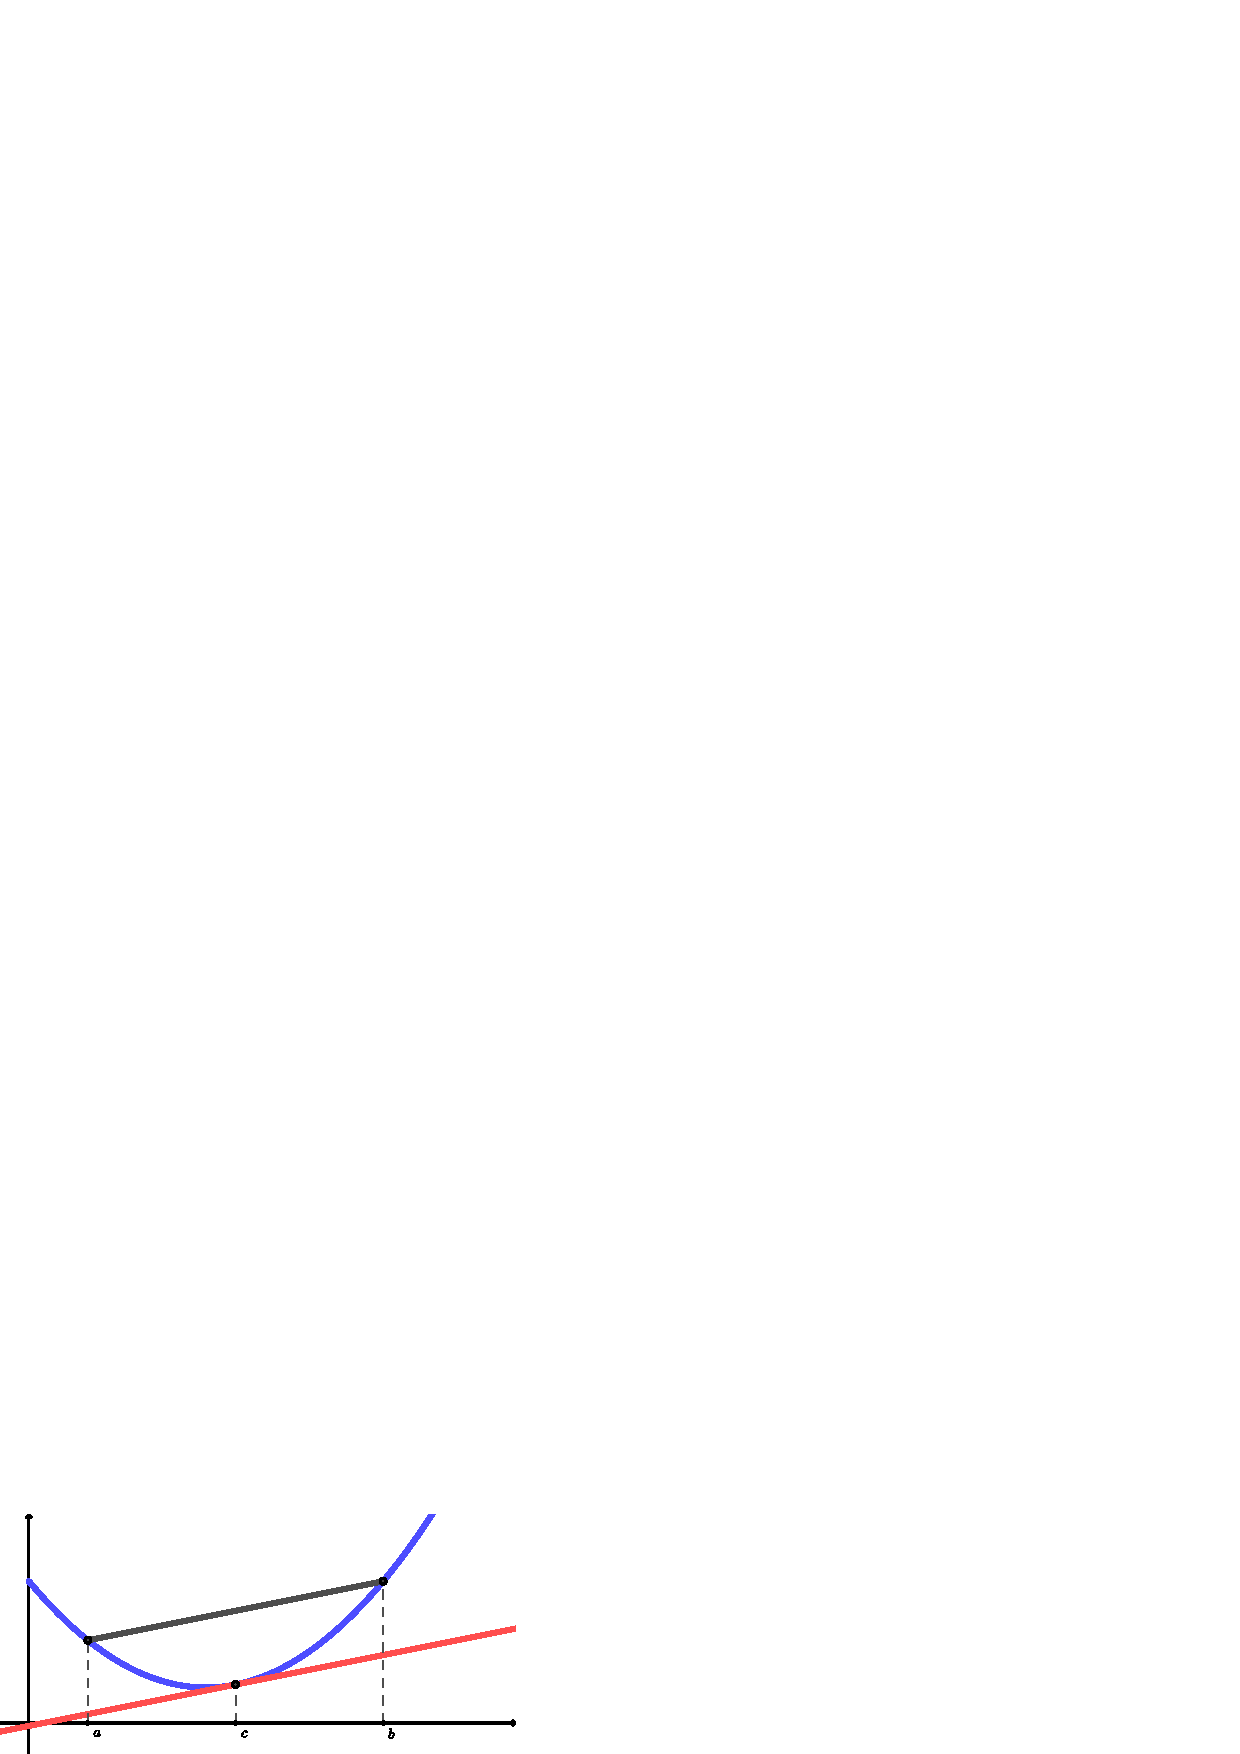
\includegraphics[width=0.5\linewidth]{./cap_derivada/valormedio.png}
\end{center}


A versão moderna deste resultado aparece no trabalho de Cauchy em 1823, embora versões preliminares tenham aparecido anteriormente (ver \href{https://en.wikipedia.org/w/index.php?title=Mean_value_teorema&oldid=824327691}{wikipedia.org/meanvalue}).


A versão em dimensões maiores deste resultado é uma desigualdade, que, como veremos, segue da definição da norma de operadores (ou, se preferir, no caso $n=1$ é a desigualdade de Cauchy-Schwarz). O resultado seguinte segue a filosofia de passar para o caso de uma variável real por meio de um caminho unidimensional (por exemplo, um segmento).

\begin{teo}[Desigualdade do Valor Médio]\label{thm:dvm}
	Seja $f:U \subseteq \mathbb{R}^n \to \mathbb{R}^m$ uma aplicação diferenciável no aberto $U$ e sejam $x, y \in U$ de modo que o segmento $[x,y]$ também está contido em $U$. Então, existe $c \in [x,y]$ tal que
	\begin{equation}\label{eqn:dvm}
	\big|f(y) - f(x)\big| \le \big\|f'(c)\big\| \cdot |y-x|.
	\end{equation}
\end{teo}

\begin{proof}
	Inicialmente mostramos o caso especial $n=1$. Neste caso, podemos supor que $U = [a,b] \subseteq \mathbb{R}$. Definimos $\phi: U \to \mathbb{R}$ por
	\[
	\phi(t) = \langle f(t), f(y) - f(x) \rangle.
	\] Pelo Teorema do Valor Médio (Teorema \ref{thm:tvm} acima) e pela Desigualdade de Cauchy-Schwarz, existe $c \in (x,y)$ tal que
	\[
	\begin{split}
	\big|f(y) - f(x)\big|^2 & = \phi(y) - \phi(x) \\
	& = \phi'(c) (y-x) \\
	& = \langle f'(c), f(y) - f(x) \rangle (y-x) \\
	& \le \big|f'(c)\big| \cdot \big|f(y) - f(x)\big| \cdot |y-x|,
	\end{split}
	\] que é equivalente a \eqref{eqn:dvm} no caso $n=1$.
	
	Para o caso geral, consideramos uma parametrização do segmento entre $x$ e $y$ e recaimos no caso que já mostramos: definimos $\alpha: [0,1] \to \mathbb{R}^m$ por
	\[
	\alpha(t) = f \big( (1-t)x + ty \big).
	\] Assim, existe $t_0 \in (0,1)$ tal que $|\alpha(1) - \alpha(0)| \le |\alpha'(t_0)|$. Pela regra da cadeia, isto é o mesmo que
	\[
	\big|f(y) - f(x)\big| \le \big| f'\big( (1-t_0)x + t_0 y \big) \cdot (y-x)\big|.
	\] O resultado segue da definição da norma de operadores, definindo $c = (1-t_0)x + t_0 y$.
\end{proof}


\begin{exer}
	Prove o Teorema \ref{thm:dvm} diretamente por integração. É necessário adicionar alguma hipótese para formalizar esta demonstração?
\end{exer}


\begin{exer}
	Verique que o Teorema do Valor Médio se estende (com igualdade) para funções escalares $f: \mathbb{R}^n \to \mathbb{R}$.
\end{exer}


\section{Segunda derivada}

Considere $f: U \to \mathbb{R}^m$ uma função diferenciável. Nós dizemos que $f$ é \textbf{duas vezes diferenciável} em $x_0$ quando $f' : U \to \mathcal{L}(\mathbb{R}^n, \mathbb{R}^m)$ é diferenciável em $x_0$. Mais explicitamente, quando existe uma transformação linear (que denotaremos por)
\begin{equation}\label{eqn:f''}
f''(x_0): \mathbb{R}^n \to \mathcal{L}(\mathbb{R}^n, \mathbb{R}^m)
\end{equation} que satisfaz
\[
\lim_{h \to 0}   \frac{\big\|f'(x_0 + h) - f'(x_0) - f''(x_0) \cdot h\big\|}{|h|} = 0.
\] Observe que a norma do numerador acima é a norma de operadores em $\mathcal{L}(\mathbb{R}^n, \mathbb{R}^m)$:
\[
T \in \mathcal{L}(\mathbb{R}^n, \mathbb{R}^m) \rightsquigarrow \|T\| := \sup_{|x|=1} \big|T(x)\big|.
\]

\begin{exer}\label{exc:lin-bilin}
	Defina
	\[
	\mathcal{B}(\mathbb{R}^n; \mathbb{R}^m) = \{ B: \mathbb{R}^n \times \mathbb{R}^n \to \mathbb{R}^m ; ~B \ \text{ é bilinear}\}
	\] e mostre que 
	\[
	\begin{split}
	\Phi: & \ \mathcal{L}\big( \mathbb{R}^n, \mathcal{L}(\mathbb{R}^n, \mathbb{R}^m) \big) \to \mathcal{B}(\mathbb{R}^n; \mathbb{R}^m) \\
	& \qquad  \qquad  T \qquad \ \ \quad \mapsto   \Phi(T)[x,y] := T(x)(y)
	\end{split}
	\] é um isomorfismo de espaços vetoriais. 
\end{exer}

O exercício acima mostra que podemos considerar $f''(x_0) \in \mathcal{B}(\mathbb{R}^n; \mathbb{R}^m)$, ou seja, $f''(x_0)$ pode tanto ser vista como uma aplicação linear do tipo \eqref{eqn:f''} quanto como uma transformação bilinear do tipo
\[
f''(x_0): \mathbb{R}^n \times \mathbb{R}^n \to \mathbb{R}^m.
\] Qualquer destas interpretações é chamada de \textbf{derivada segunda} de $f$ em $x_0$. Tem-se, usando a identificação do Exercício \ref{exc:lin-bilin},
\[
f''(x_0) (v,w) = f''(x_0) (v)(w) = \frac{\partial}{\partial w} \left( f'(x_0) (v) \right) = \frac{\partial}{\partial w} \left( \frac{\partial f}{\partial v} \right) (x_0).
\] Vamos utilizar a notação mais comum 
\[
f''(x_0) (v,w) = \frac{\partial^2 f}{\partial w \ \partial v} (x_0).
\]

\begin{exer}
	Escrever $f''(x_0) (v,w)$ em coordenadas. Dados $v = \sum_{i=1}^n v^i e_i$ e $w = \sum_{i=1}^n w^i e_i$, obter as $m$ componentes de $f''(x_0) (v,w) \in \mathbb{R}^m$.
\end{exer}


Prosseguindo como acima, define-se a terceira derivada em $x_0$ como uma forma trilinear e assim por diante. Além disso, dizemos que 
\begin{itemize}
	\item $f$ é de classe $C^0$ quando é contínua;
	
	\item $f$ é de classe $C^1$ quando $f$ é diferenciável e $f'$ é contínua;
	
	\item $f$ é de classe $C^2$ quando $f$ e $f'$ são diferenciáveis e $f''$ é contínua;
	
	\item[] $\qquad \vdots$
	
	\item $f$ é de classe $C^{\infty}$ quando existem as derivadas de todas as ordens de $f$.
\end{itemize}


A diferenciabilidade de composições de funções acontece de acordo com a \textbf{regra da cadeia}: para $f: \mathbb{R}^n \to \mathbb{R}^m$ e $g: \mathbb{R}^m \to \mathbb{R}^p$ diferenciáveis,
\[
(g \circ f)' (x_0) = g' \big( f(x_0) \big) \cdot f'(x_0),
\] ou, em componentes, para $i = 1,2, \dots, p$ e $j = 1, 2, \dots, n$,
\[
\frac{\partial}{\partial x_j} g_i \big( f(x_0) \big) = \sum_{k=1}^{m} \frac{\partial g_i}{\partial y_k}\big( f(x_0) \big) \frac{\partial f_k}{\partial x_j} (x_0).
\]






\section{Fórmula de Taylor}


A Fórmula de Taylor unidimensional nos diz que se $f: \mathbb{R} \to \mathbb{R}$ é uma função de classe $C^{k+1}$, então existe $\xi$ no intervalo aberto entre $a$ e $x$ tal que
\[
f(x) = f(a) + f'(a) (x-a) + \frac{f''(a)}{2!} (x-a)^2 + \cdots + \frac{f^{(k)}(a)}{k!} (x-a)^k + \frac{f^{(k+1)}(\xi)}{(k+1)!} (x-a)^{k+1}.
\]

Vamos obter uma versão multidimensional deste resultado. 

\begin{teo}[Fórmula de Taylor]
	Suponhamos que $f: \mathbb{R}^n \to \mathbb{R}$ é uma função de classe $C^{k+1}$ em uma bola $B_r(a)$, então, para $x \in B_r(a) \subseteq \mathbb{R}^n$, existe $\xi$ no segmento de $a$ para $x$ tal que
	\begin{equation}\label{eqn:taylor}
	f(x) = f(a) + f'(a) \cdot (x-a) + \cdots + \frac{1}{k!} f^{(k)}(a) \cdot (x-a)^k + \frac{1}{(k+1)!} f^{(k+1)}(\xi) \cdot (x-a)^{k+1}.
	\end{equation}
\end{teo}

A notação do Teorema deveria ser, mais precisamente,
\[
f^{(j)}(a) (x-a, x-a, \dots, x-a) \ \text{ ao invés de } \ f^{(j)}(a) \cdot (x-a)^j,
\] pois estamos pensando em $f^{(j)}(a)$ como uma aplicação $j$-linear.

\begin{proof}
	Como já fizemos na prova da Desigualdade do Valor Médio, vamos nos restringir ao segmento de reta que une $a$ a $x$ e aplicar o caso conhecido unidimensional. Já que quremos considerar $t=0$ e $t=1$, escolhemos $\delta > 0$ adequado e definimos $\phi: [-\delta,1+\delta] \to \mathbb{R}$ por
	\[
	\phi(t) = f \big( (1-t)a + tx \big) = f \big( a + t(x-a) \big).
	\] A fórmula de Taylor unidimensional implica que existe $\tau \in (0,1)$ de modo que
	\begin{equation}\label{eqn:taylor-phi}
	\phi(1) = \phi(0) + \phi'(0) + \cdots + \frac{1}{k!} \phi^{(k)}(0) + \frac{1}{(k+1)!} \phi^{(k+1)}(\tau).
	\end{equation} O resultado segue da Regra da Cadeia, com $\xi =a + \tau(x-a)$.
\end{proof}


Para escrever mais explicitamente a fórmula de Taylor em termos de derivadas parciais de $f$, vamos introduzir uma notação adicional. Um \textbf{multi-índice} é um elemento $\alpha \in \mathbb{N}^n$ que, para os nossos propósitos, representa o número de derivadas parciais com respeito à variável que está na respectiva posição. Por exemplo, para $f:\mathbb{R}^5 \to \mathbb{R}$, denotamos 
\[
\frac{\partial^5 f}{\partial x_3^3 \partial x_2 \partial x_4} (a) = D^\alpha f (a), \quad \text{onde} \quad \alpha = (0, 3,2,1, 0).
\] Também é comum utilizar multi-índices para denotar produtos das componentes de um vetor:
\[
x^\alpha = x_2^3 x_3^2 x_4, \quad \text{onde} \quad \alpha = (0,3,2,1,0).
\] Para simplificar a notação, é também comum escrever
\[
|\alpha| = \alpha_1 + \alpha_2 + \cdots + \alpha_n, \qquad \alpha! = \alpha_1 ! \alpha_2 ! \cdots  \alpha_n! \quad \text{e} \quad 
\binom{n}{\alpha} = \frac{n!}{\alpha!} = \frac{n!}{\alpha_1 ! \alpha_2 ! \cdots  \alpha_n!}.
\]


\begin{exer}(Teorema Multinomial)
	Mostre que, para $N \in \mathbb{N}$ fixado e $a_1, a_2, \dots a_k \in \mathbb{R}$, vale
	\[
	(a_1 + a_2 + \cdots + a_k)^N = \sum_{\alpha_1 + \alpha_2 + \cdots + \alpha_n = N} \frac{N!}{\alpha_1 ! \alpha_2 ! \cdots  \alpha_k!} a_1^{\alpha_1} a_2^{\alpha_2} \cdots  a_k^{\alpha_k}.
	\] Na notação introduzida acima, podemos escrever, mais sucintamente,
	\[
	(a_1 + a_2 + \cdots + a_k)^N = \sum_{|\alpha|  = N} \binom{N}{\alpha} a^\alpha, \quad \text{onde} \quad a = (a_1, a_2, \dots, a_k).
	\] \underline{\textit{Dica}}: Mostrar o caso $k=2$, conhecido como binômio de Newton, e depois fazer indução em $k$.
\end{exer}

Agora, vamos utilizar o Teorema Multinomial para calcular \eqref{eqn:taylor-phi} mais explicitamente. Iniciamos observando que
\[
\phi'(t) = \frac{\mathrm{d} }{\mathrm{d}  t} f(a + t v) = v_1 \frac{\partial f}{\partial x_1} + v_2 \frac{\partial f}{\partial x_2} + \cdots + v_n \frac{\partial f}{\partial x_n} = \left( v_1 \frac{\partial }{\partial x_1} + v_2 \frac{\partial }{\partial x_2} + \cdots + v_n \frac{\partial }{\partial x_n}  \right) f.
\] Logo, utilizando o Teorema Multinomial,
\[
\phi^{(j)}(t) = \left( v_1 \frac{\partial }{\partial x_1} + v_2 \frac{\partial }{\partial x_2} + \cdots + v_n \frac{\partial }{\partial x_n}  \right)^{j} f = \sum_{|\alpha| = n} \frac{j!}{\alpha!} v^\alpha D^{\alpha} f (a + tv).
\] Portanto, \eqref{eqn:taylor} é o mesmo que
\[
f(x) = \sum_{|\alpha| \le k} \frac{1}{\alpha!} (x-a)^\alpha D^{\alpha} f (a) + \sum_{|\alpha| = k+1} \frac{1}{\alpha!} (x-a)^\alpha D^{\alpha} f (\xi).
\]


\subsection{Caso especial $k=2$; Hessiana}

Para a maior parte das aplicações, é suficiente escrever a fórmula de Taylor até ordem 2 apenas. Além disso, observamos que, a partir da forma bilinear $f''(a): \mathbb{R}^n \times \mathbb{R}^n \to \mathbb{R}$, podemos definir uma forma quadrática $Q(v) = f''(a) (v,v)$. Esta forma quadrática é conhecida como a \textbf{Hessiana} de $f$ em $a$. Vejamos qual é a matriz simétrica associada à Hessiana: escrevendo $v$ na base canônica,
\[
Q(v) = f''(a) (v,v) = \frac{\partial^2 f}{\partial v^2} (a) = \sum_{i=1}^{n} \frac{\partial^2 f}{\partial x_i \partial x_j} (a) v_i v_j = \langle \nabla^2 f (a) v, v \rangle = v^T \nabla^2 f (a) v,
\] onde $\nabla^2 f (a)$ é a matriz das derivadas de ordem 2 de $f$:
\[
\nabla^2 f (a) = 
\begin{bmatrix}
\frac{\partial^2 f}{\partial x_i \partial x_j} (a)
\end{bmatrix}_{n \times n}.
\] Por abuso de linguagem, $\nabla^2 f (a)$ é também conhecida como a Hessiana de $f$ em $a$.

Com esta nova notação, enunciamos um caso particular da Fórmula de Taylor que provamos:

\begin{corol}
	Suponhamos que $f: \mathbb{R}^n \to \mathbb{R}$ é uma função de classe $C^{3}$ em uma bola $B_r(a)$, então, para $x \in B_r(a) \subseteq \mathbb{R}^n$, existe $\xi$ no segmento de $a$ para $x$ tal que
	\begin{equation}
	f(x) = f(a) + \nabla f(a) \cdot (x-a) + \frac{1}{2} (x-a)^T \nabla^2 f (a) (x-a) + r(x-a),
	\end{equation} onde 
	\[
	\lim_{x\to a} \frac{r(x-a)}{|x-a|^2} = 0.
	\]
\end{corol}


\begin{exer}
	Verifique que é válido o corolário acima. É realmente necessário $f \in C^3$?
\end{exer}



\section{Problems de otimização - máximos e mínimos}


Nesta seção, estudamos condições necessárias e suficientes para que um ponto $a \in \mathbb{R}^n$ seja um minimizante (ou maximizante) para $f: \mathbb{R}^n \to \mathbb{R}$. Começamos com uma condição necessária de ordem um.

\begin{prop}
	Suponhamos que $a \in \operatorname{int} U$ é um ponto de mínimo local de $f: U \subseteq \mathbb{R}^n \to \mathbb{R}$ e que $f$ é diferenciável em $a$. Então, $\mathrm{d}  f(a) = 0$.
\end{prop}

\begin{proof}
	Utilizando que $a$ é mínimo local e a definição de diferenciabilidade, temos que para todo $v$ próximo da origem:
	\[
	f(a) \le f(a+v) = f(a) + \mathrm{d}  f(a) \cdot v + r(v) \quad \text{e também} \quad \frac{r(v)}{|v|} \to 0.
	\] Dividindo pelo comprimento de $v$ e fazendo $v \to 0$, concluimos que $\mathrm{d}  f(a) \cdot w \ge 0$ para todo $w$ unitário. Em particular, podemos trocar $w$ por $-w$ e segue que $\mathrm{d}  f(a) =0$.
\end{proof}

Um ponto $a \in \mathbb{R}^n$ é dito \textbf{ponto crítico} de $f$ quando $\mathrm{d}  f(a) = 0$. Assim, o teorema acima afirma que todo extremizante de $f$ é ponto crítico. A recíproca não é verdadeira: $a = 0$ é ponto crítico de $f(x) = x^3$ que não é de mínimo nem de máximo.


Lembramos que uma matriz $A$ de ordem $n \times n$ é dita \textbf{positiva definida} quando 
\[
\langle A v, v  \rangle \ge 0 \quad \text{para todo } v \in \mathbb{R}^n.
\] É comum a notação $A \ge 0$. A matriz $A$ é dita \textbf{estritamente positiva definida}, e se escreve $A > 0$, quando
\[
\langle A v, v  \rangle > 0 \quad \text{para todo } v \in \mathbb{R}^n.
\]


\begin{prop}\label{prop:neces2}
	Suponhamos que $a \in \operatorname{int} U$ é um ponto de mínimo local de $f: U \subseteq \mathbb{R}^n \to \mathbb{R}$ e que $f$ é duas vezes diferenciável em $a$. Então, a matriz Hessiana $\nabla^2 f (a)$ é positiva definida:
	\[
	\langle \nabla^2 f (a) v, v  \rangle \ge 0 \qquad \text{para todo } v \in \mathbb{R}^n.
	\]
\end{prop}

\begin{proof}
	Pela proposição anterior, $\nabla f (a) = 0$. Logo, pela fórmula de Taylor, temos que
	\[
	f(a) \le f(a + h) = f(a) + \frac{1}{2} \langle \nabla^2 f (a) \cdot h, h \rangle + r(h),
	\] para todo $h \in B_{\delta} (0)$ próximo de zero (já que $a$ é um ponto de mínimo local). Segue que
	\[
	\langle \nabla^2 f (a) \cdot h, h \rangle + 2 r(h) \ge 0.
	\] Dividindo por $|h|^2$ e fazendo $h \to 0$, concluimos que
	\[
	\langle \nabla^2 f (a) w, w  \rangle \ge 0 \qquad \text{para todo vetor unitário}\quad  w \in \mathbb{R}^n.
	\] Para concluir a demonstração, basta fazer $w = v /|v|$ e multiplicar por $|v|^2$.
\end{proof}


\begin{exer}
	A recíproca da Proposição \ref{prop:neces2} não é verdadeira; encontre um contra-exemplo. Enuncie e prove resultados análogos às duas proposições acima para pontos de máximo local.
\end{exer}

Se tivermos uma matriz Hessiana estritamente positiva, daí sim a recíproca é verdadeira.


\begin{prop}\label{prop:neces3}
	Seja $f: U \subseteq \mathbb{R}^n \to \mathbb{R}$ de classe $C^2$ em $U$. Suponhamos que
	\begin{itemize}
		\item $\nabla f (a) = 0$ e
		
		\item $\nabla^2 f(a) > 0$.
	\end{itemize} Então, $a$ é um ponto de mínimo local estrito para $f$.
\end{prop}

\begin{proof}
	Assim como na Proposição \ref{prop:neces2} acima, utilizamos a Fórmula de Taylor:
	\[
	f(a + h) = f(a) + \frac{1}{2} \langle \nabla^2 f (a) \cdot h, h \rangle + r(h)  \quad \text{onde} \quad \lim_{h \to 0} \frac{r(h)}{|h|^2} = 0.
	\] Dividindo por $|h|^2$ podemos escrever
	\[
	\frac{f(a + h) - f(a)}{|h|^2} = \frac{1}{2} \left\langle \nabla^2 f (a) \cdot \frac{h}{|h|}, \frac{h}{|h|} \right\rangle + \rho(h)  \quad \text{onde} \quad \lim_{h \to 0} \rho(h) = 0.
	\] A aplicação $w \mapsto \langle \nabla^2 f (a) \cdot w, w \rangle$ assume um mínimo positivo na esfera unitária, de modo que, para algum $C>0$, vale que
	\[
	\frac{f(a + h) - f(a)}{|h|^2} \ge C + \rho(h)  \quad \text{onde} \quad \lim_{h \to 0} \rho(h) = 0.
	\]
	Agora, existe $\delta >0$ tal que
	\[
	h \in B_{\delta}(0) \implies C + \rho(h) > 0,
	\] concluindo a demonstração.
\end{proof}


\begin{exer}\label{prop:neces4}
	Adaptar o raciocínio acima para pontos de máximo local de $f$.
\end{exer}


\begin{prop}
	Seja $f: U \subseteq \mathbb{R}^n \to \mathbb{R}$ de classe $C^2$ em $U$. Suponhamos que
	\begin{itemize}
		\item $\nabla f (a) = 0$ e
		
		\item $\nabla^2 f(a)$ é \textbf{indefinida}: $\langle \nabla^2 f(a) v, v \rangle$ muda de sinal.
	\end{itemize} Então, $a$ não é nem um ponto de mínimo local nem um ponto de máximo local para $f$.
\end{prop}

\begin{proof}
	O argumento utilizado nas demonstrações da Proposição \ref{prop:neces3} e do Exercício \ref{prop:neces4} mostra que, para $h$ suficientemente próximo da origem,
	\[
	\frac{f(a + h) - f(a)}{|h|^2} \ \text{ tem o mesmo sinal de }\ \left\langle \nabla^2 f (a) \cdot \frac{h}{|h|}, \frac{h}{|h|} \right\rangle.
	\] Isto conclui a prova da proposição.
\end{proof}


É um exercício de Álgebra Linear mostrar que uma matriz $A$ é positiva definida se, e somente se, todos os seus autovalores são positivos.

\begin{exer}
	Faça o exercício!
\end{exer}

Mas pode ser bastante trabalhoso encontrar todos os autovalores de $A$. Um método indireto consiste em completar quadrados até se ``livrar" dos termos mistos da forma quadrática $\langle Av, v\rangle$. Vejamos um exemplo.

\begin{ex}
	Considere
	\[
	A = 
	\begin{bmatrix}
	1 & 2 & 0 \\
	2 & 1 & 1 \\
	0 & 1 & -2 
	\end{bmatrix}
	\] de modo que 
	\[
	\langle Ax, x\rangle = x_1^2 + x_2^2 - 2x_3^2 + 4 x_1 x_2 + 2 x_2 x_3.
	\] Juntando os termos que têm $x_1$, obtemos
	\[
	x_1^2 + 4 x_1 x_2 = (x_1 + 2x_2)^2 - 4 x_2^2 =: a^2 - 4x_2^2 \quad \text{onde} \quad a = x_1 + 2x_2.
	\] Logo,
	\[
	\langle Ax, x\rangle = a^2 - 3 x_2^2 - 2x_3^2 + 2 x_2 x_3.
	\] Em seguida, juntando os termos com $x_2$:
	\[
	- 3 x_2^2 + 2 x_2 x_3 = - 3 \left(x_2^2 + \frac{2}{3} x_2 x_3 \right) = - 3 \left(x_2 + \frac{x_3}{3} \right)^2 + \frac{x_3^2}{3} =: -3 b^2 + \frac{x_3^2}{3} \quad \text{onde} \quad b = x_2 + \frac{x_3}{3}.
	\] Denotando $c = x_3$, obtemos
	\[
	\langle Ax, x\rangle = a^2 + -3b^2 + \frac{c^2}{3}.
	\] Desta forma, é fácil ver que $\langle Ax, x\rangle$ assume tanto valores positivos quanto negativos; basta escolher alguns valores baseados nos sinais que aparecem nos termos ao quadrado. Por exemplo, quando $b = 0$, temos valores positivos. Quando $a = c = 0$, temos valores negativos. Portanto, $A$ é uma matriz indefinida.
\end{ex}


\section{Funções Convexas}

Funções convexas são dos objetos mais importantes em matemática, principalmente em problems de otimização do cálculo de variações. A referência mais clássica para o assunto é Rockafellar \cite{Rock-97}. O material desta seção é uma ampliação de Villani \cite[Subseção 2.1.3]{Vill-03}, que já é bastante inspirado em \cite{Rock-97}. No entanto, não vamos nos aprofundar nos tópicos que necessitam de Teoria da Medida, para não fugir dos pré-requisitos do nosso curso.


Uma função $f: \mathbb{R}^n \to \mathbb{R}\cup \{+ \infty\}$ é uma \textbf{função convexa própria}\footnote{No contexto de Análise Convexa, a palavra \textit{própria} indica que $f > - \infty$ em todo ponto e que $f(x) < + \infty$ para pelo menos um ponto \cite[Seção 4]{Rock-97}.} quando $f$ não é identicamente $+ \infty$ e, para todo $x,y \in \mathbb{R}^n$ e para todo $0<\lambda<1$, tem-se
\begin{equation}\label{eqn:convex}
f \big[ (1-\lambda)x + \lambda y \big] \le (1-\lambda) f(x) + \lambda f(y).
\end{equation} Quando a desigualdade é estrita em \eqref{eqn:convex}, dizemos que $f$ é \textbf{estritamente convexa}.

O \textbf{domínio efetivo} de uma função convexa $f$ é o conjunto
\[
\operatorname{dom} f := \big\{ x \in \mathbb{R}^n ; ~f(x) < + \infty \big\}.
\] É fácil de ver que $\operatorname{dom} f$ é um conjunto convexo (exercício). É também fácil ver que:

\begin{exer}(Desigualdade de Jensen - versão discreta)
	A função $f : \mathbb{R}^n \to \mathbb{R}\cup \{+ \infty\}$ é convexa se, e somente se, para todo $\lambda_1\ge 0, \lambda_2 \ge 0, \dots, \lambda_m \ge 0$ com $\lambda_1 + \lambda_2 + \cdots + \lambda_m = 1$, temos
	\[
	f \big[\lambda_1 x_1 + \lambda_2 x_2 + \cdots + \lambda_m x_m \big] \le \lambda_1 f(x_1) + \lambda_2 f(x_2) + \cdots + \lambda_m f(x_m).
	\]
\end{exer}

Uma propriedade geométrica que segue da definição é que o gráfico de uma função convexa está ``acima'' do plano tangente em cada um dos pontos de diferenciabilidade:

\begin{prop}\label{prop:convex-planosuporte}
	Se $f: \mathbb{R}^n \to \mathbb{R}\cup \{+ \infty\}$ é uma função convexa própria que é diferenciável em $x \in \operatorname{dom} f$, então
	\[
	f(y) \ge f(x) + \langle \nabla f (x), y-x \rangle,
	\] para todo $y \in \mathbb{R}^n$. Em particular, $\nabla f$ é monótono em pontos de diferenciabilidade:
	\[
	\langle \nabla f(y) - \nabla f(x), y-x \rangle \ge 0.
	\]
\end{prop}

\begin{proof}
	Reescrevendo \eqref{eqn:convex} como
	\[
	\frac{f \big[ x + \lambda (y-x) \big] - f(x)}{\lambda} \le f(y) - f(x)
	\] e mandando $\lambda \to 0$, obtemos o resultado.
\end{proof}

Na verdade, esta propriedade de o gráfico estar acima dos planos tangentes caracteriza funções convexas:

\begin{prop}\label{prop:convex-planosuporte2}
	Suponhamos que $f: \mathbb{R}^n \to \mathbb{R} \cup \{+ \infty\}$ é uma função de classe $C^1$ que satisfaz
	\[
	f(y) \ge f(x) + \langle \nabla f (x), y-x \rangle,
	\] para todo $x, y \in \mathbb{R}^n$. Então $f$ é uma função convexa.
\end{prop}

\begin{proof}
	É sempre verdade que (como se vê tomando $x = y$)
	\[
	f(y) \le \sup_{x \in \mathbb{R}^n} \Big[ f(x) + \langle \nabla f (x), y-x \rangle \Big].
	\] Logo, nossa hipótese garante que, na verdade,
	\[
	f(y) = \sup_{x \in \mathbb{R}^n} \Big[ f(x) + \langle \nabla f (x), y-x \rangle \Big].
	\] O resultado segue da observação que o supremo pontual de uma família qualquer de funções convexas é também uma função convexa.
\end{proof}

\begin{exer}
	Mostre que o supremo pontual de uma família qualquer de funções convexas é também uma função convexa, isto é, dadas $f_\lambda$ convexas, temos que 
	\[
	f(y) := \sup_{\lambda \in \Lambda} f_\lambda (y)
	\] é convexa.
\end{exer}

Em seguida, mostramos outra caracterização de funções convexas, mas com derivadas de ordem dois.

\begin{prop}\label{thm:convex-hessian}
	Seja $f: \mathbb{R}^n \to \mathbb{R}\cup \{+ \infty\}$ é uma função de classe $C^2$. Então $f$ é convexa se, e somente se, $\nabla^2 f (x)$ é positiva semi-definida, para todo $x \in \operatorname{dom} f$, isto é, 
	\[
	\langle \nabla^2 f (x) y , y\rangle \ge 0,
	\] para todo $x, y \in \mathbb{R}^n$.
\end{prop}

\begin{proof}
	$\boxed{\stackrel{\hspace{0.2cm}}{\implies}}\ $ Como $x = \frac{x + ty}{2} + \frac{x - ty}{2}$, a definição de função convexa implica que
	\[
	2 f(x) \le f(x + ty) + f(x-ty).
	\] Logo,
	\[
	\frac{f(x + ty) + f(x-ty) - 2 f(x)}{t^2} \ge 0.
	\] Fazendo $t \to 0$, obtemos o que queríamos.
	
	$\boxed{\stackrel{\hspace{0.2cm}}{\impliedby}}\ $ Pelo Teorema do Valor Médio, para todo $x,y \in \mathbb{R}^n$,
	\[
	f(y) - f(x) =  \langle \nabla f (x), y - x \rangle + \frac{\big\langle \nabla^2 f (\xi) \,  (y-x), y - x \big\rangle}{2} \ge \langle \nabla f (x), y - x \rangle.
	\]		
	
	Uma outra forma de provar (que também é a ideia da prova da Fórmula de Taylor com resto integral) é fazer duas aplicações do Teorema Fundamental do Cálculo:
	\[
	\begin{split}
	f(y) - f(x) & = \int_0^1 \frac{\mathrm{d} }{\mathrm{d}  t} f \Big[ x  + t(y-x) \Big] \, \mathrm{d}  t \\
	& = \int_0^1 \langle \nabla f \big[ x  + t(y-x) \big], y - x \rangle \, \mathrm{d}  t \\            
	& = \langle \nabla f (x), y - x \rangle + \left\langle \int_0^1  \Big[\nabla f \big[ x  + t(y-x)  \big] - \nabla f (x)\Big]  \, \mathrm{d}  t, y - x \right\rangle \\
	& = \langle \nabla f (x), y - x \rangle + \left\langle \int_0^1  \int_0^1 \frac{\mathrm{d} }{\mathrm{d}  s} \nabla f \big[ x  + s t(y-x)  \big] \, \mathrm{d}  s \, \mathrm{d}  t, y - x \right\rangle \\
	& = \langle \nabla f (x), y - x \rangle + \left\langle \int_0^1  \int_0^1 \nabla^2 f \big[ x  + s t(y-x)  \big] \, \Big( t (y-x) \Big) \, \mathrm{d}  s \, \mathrm{d}  t, y - x \right\rangle \\
	& = \langle \nabla f (x), y - x \rangle + \int_0^1 \int_0^1 t \, \Big\langle \nabla^2 f \big[ x  + s t(y-x)  \big] \,  (y-x), y - x \Big\rangle  \, \mathrm{d}  s \, \mathrm{d}  t \\
	& \ge \langle \nabla f (x), y - x \rangle. \qedhere
	\end{split}
	\]
\end{proof}

\subsection{Regularidade de primeira ordem}

A questão seguinte de nosso interesse é a análise da regularidade de funções convexas. Por exemplo, dada uma função convexa própria,
\begin{itemize}
	\item será $f$ contínua?
	\item será $f$ diferenciável?
\end{itemize} Passamos a estudar estas questões.

\begin{teo}\label{thm:convex-loclip}
	Suponhamos que $f: \mathbb{R}^n \to \mathbb{R}\cup \{+ \infty\}$ é uma função convexa própria. Então, $f$ é localmente limitada e localmente Lipschitz em $\operatorname{int} (\operatorname{dom} f)$. Em particular\footnote{O Teorema de Rademacher afirma que funções Lipschitz são diferenciáveis em quase todo ponto.}, $f$ é diferenciável em quase todo ponto de $\operatorname{dom} f$.
\end{teo}

Vamos apresentar duas provas de que funções convexas são localmente de Lipschitz. A primeira vale apenas em dimensão um, mas é bastante instrutiva. A segunda é uma prova em dimensão $n \ge 1$ que é também elementar.

\begin{proof}[Demonstração em dimensão 1]
	Se $n=1$, $\operatorname{int} \operatorname{dom} f$ é um intervalo $(a,b)$. Em dimensão um, é possível caracterizar funções convexas como: dados $a < x < b$, temos
	\begin{equation}\label{eqn:convex1d}
	\frac{f(x) - f(a)}{x-a} \le \frac{f(b) - f(a)}{b-a} \le \frac{f(b) - f(x)}{b-x}.
	\end{equation} Para ver isso, tomamos $t = \frac{x-a}{b-a} \in (0,1)$ de modo que $x = (1-t)a + t b$. Logo,
	\[
	f(x) \le (1- t) f(a) + t f(b) = f(a) + \frac{f(b) - f(a)}{b - a} (x-a).
	\] Então,
	\[
	\frac{f(x) - f(a)}{x-a} \le \frac{f(b)-f(a)}{b-a}.
	\] Considerando $s \in (0,1)$ tal que $x = sa + (1-s) b$, conseguimos a segunda desigualdade em \eqref{eqn:convex1d}.
	
	Considere $(c,d) \subset\subset (a,b)$. Iterando \eqref{eqn:convex1d}, temos que, para $a < c < x < y < d < b$,
	\[
	\frac{f(c) - f(a)}{c-a} \le \frac{f(y) - f(x)}{y-x} \le \frac{f(b) - f(d)}{b-d}.
	\] Escolhendo 
	\[
	M := \max \left\{ \left| \frac{f(c) - f(a)}{c-a} \right|, \left| \frac{f(b) - f(d)}{b-d} \right| \right\},
	\] temos $\big|f(y) - f(x)\big| \le M |x-y|$, para quaisquer $x,y \in (c,d).$
\end{proof}

Finalmente, apresentamos uma segunda prova de que $f$ é localmente Lipschitz.

\begin{proof}[Demonstração]
	Considere $x_0 \in \operatorname{int} \operatorname{dom} f$ e $Q_r(x_0) \subset \operatorname{int} \operatorname{dom} f$ um cubo fechado centrado em $x_0$ cujas arestas tem comprimento $2r$ e são paralelas com os eixos coordenados. Observe que $B_r(x_0) \subset Q_r(x_0)$. Sendo $f$ convexa, o máximo de $f$ em $Q_r(x_0)$ é atingido em um dos vértices $x_k$ do cubo (exercício). Logo,
	\[
	f(y) \le \sup_k f(x_k) =:M < + \infty, \ \text{ para todo } \ y \in B_r(x_0).
	\]
	
	Em seguida, vamos mostrar que $f$ é também limitada por baixo em $B_{r} (x_0)$. De fato, dado $x \in B_{r} (x_0)$, temos que $y := 2x_0 - x \in B_r(x_0)$. Logo,
	\[
	x_0 = \frac{x + y}{2} \implies f(x_0) \le \frac{f(x) + f(y)}{2} \le \frac{f(x) + M}{2} \implies f(x) \ge 2 f(x_0) - M.
	\] Logo, $|f| \le C$ em $B_r(x_0)$, o que mostra que $f$ é localmente limitada em $\operatorname{int} \operatorname{dom} f$.
	
	Agora, fixamos $\delta \in (0,r)$. Dados $x, y \in B_{r - \delta}(x_0)$, temos que
	\[
	y = \frac{\delta}{\delta + \|y-x\|} \, x + \frac{\|y-x\|}{\delta + \|y-x\|} \, z, \ \text{ onde } \ z = y + \delta \frac{y-x}{\|y-x\|} \in B_r(x_0).
	\] Usando convexidade,
	\[
	f(y) \le \frac{\delta}{\delta + \|y-x\|}  f(x) + \frac{\|y-x\|}{\delta + \|y-x\|} f(z).
	\] Logo,
	\[
	f(y) - f(x) \le \frac{f(z) - f(x)}{\delta + \|y-x\|} \,  \|y-x\| \le \frac{2C}{\delta} \,  \|y-x\|.
	\] Trocando os papéis de $x,y \in B_{r - \delta}(x_0)$, concluimos que $f$ é de Lipschitz em $B_{r - \delta}(x_0)$.
\end{proof}

\subsection{Regularidade de segunda ordem -- o Teorema de Alexandrov}


Em seguida, estudamos diferenciabilidade de segunda ordem para funções convexas. O Teorema de Alexandrov diz que funções convexas são duas vezes diferenciáveis para quase todo ponto, que é um resultado notável, já que diferenciabilidade de primeira ordem é apenas quase sempre. Um pouco mais exeplicitamente, o Teorema de Alexandrov afirma que, para quase todo ponto, existe uma matriz, que pode ser chamada de ``Hessiana'', que de fato tem a ver (em um certo sentido) com derivadas de segunda ordem de $f$, e que cumpre seu papel no sentido da Fórmula de Taylor.

\begin{teo}[Teorema de Alexandrov]
	Seja $f:\mathbb{R}^n \to \mathbb{R}$ uma função convexa. Então, existe um conjunto $A$ de medida nula tal que, para todo $x \in \mathbb{R}^n \setminus A$, existe uma matriz (denotada por) $\nabla^2 f (x)$ que satisfaz
	\[
	f(x + v) = f(x) + \langle \nabla f (x), v \rangle + \frac{\langle \nabla^2 f (x) v, v  \rangle}{2} + o (|v|^2) \quad \text{quando} \quad v \to 0.
	\]
\end{teo}

\begin{proof}
	Pode ser encontrada em Evans, Gariepy \cite{EvGa-92} ou Villani \cite{Vill-09}. Necessita de conhecimentos de Teoria da Medida.
\end{proof}

\section{O Teorema da Função Inversa}

O Teorema da Função Inversa figura como um dos resultados mais importantes da análise matemática moderna. O teorema nos dá uma condição suficiente para que funções vetoriais sejam invertíveis na vizinhança de um ponto. Não é tão claro quem foi o primeiro a demonstrar este resultado, mas uma busca no Google\footnote{\href{https://mathoverflow.net/questions/94323/who-was-the-first-to-formulate-the-inverse-function-teorema/94412}{https://mathoverflow.net/questions/94323/who-was-the-first-to-formulate-the-inverse-function-teorema}, visualizado em 30 de Janeiro de 2018} mostrou que o Teorema da Função Inversa já aparecia no trabalho de Ulisse Dini\footnote{Matemático italiano que viveu de 14 de Novembro de 1845 até 28 de Outubro de 1918. Nascido em Pisa, Itália, estudou na Scuola Normale Superiore, sob orientação de Enrico Betti. Também estudou em Paris com Charles Hermite, através de bolsas de intercâmbio. É conhecido por seu trabalho em Análise Real, no perído de formulação rigorosa de vários conceitos da teoria. Seu nome aparece no Critério de Dini (para convergência de séries de Fourier), Teorema de Dini (sobre convergência de sequências monótonas de funções), é creditado o Teorema da Função Implícita, que veremos mais adiante no curso, etc. Dini faleceu aos 72 anos em Pisa, Itália. Algumas destas informações foram retiradas de \href{https://en.wikipedia.org/w/index.php?title=Ulisse_Dini&oldid=812724987}{https://en.wikipedia.org/w/index.php?title=Ulisse\underline{\hspace{0.2cm}}Dini\&oldid=812724987} em 03 de Janeiro de 2018. Segue um retrato de Dini (que também pode ser encontrado no link acima).}, em "Lezioni di Analisi Infinitesimale", de 1877. 
\begin{center}
	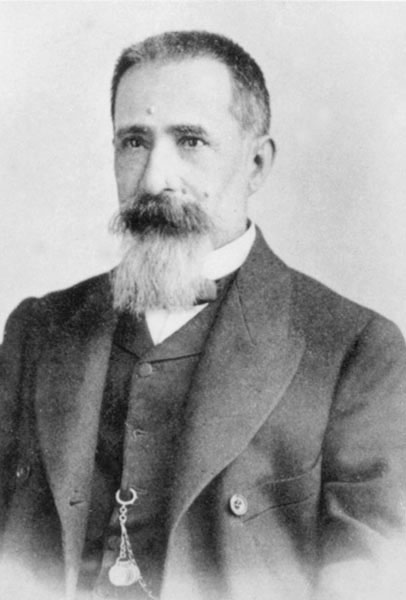
\includegraphics[width=0.3356\linewidth]{./cap_derivada/Ulisse_Dini.jpg} \ 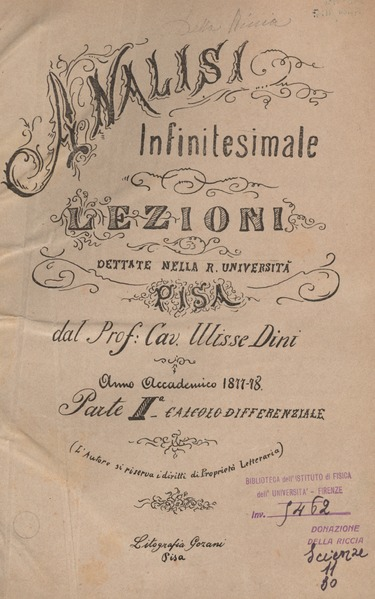
\includegraphics[width=0.31\linewidth]{./cap_derivada/Dini_-_Lezioni_di_analisi_infinitesimale,_1878.jpg}
\end{center}

\begin{teo}[Teorema da Função Inversa]
	Seja $f: E \subseteq \mathbb{R}^n \to \mathbb{R}^n$ uma função de classe $C^1(E, \mathbb{R}^n)$ e que, para algum $a \in E$, a transformação linear $f'(a)$ é invertível. Então, $f$ é invertível, com inversa diferenciável, perto do ponto $a$. 
	
	Mais precisamente, existe um aberto $U$ que contem $a$ e um aberto $V$ que contém $f(a)$ tais que
	\begin{enumerate}[$(i)$]
		\item $f$ é injetiva em $U$;
		
		\item $f(U) = V$, de modo que $f: U \to V$ é uma bijeção; 
		
		\item A inversa $f^{-1}$ é de classe $C^{1}(V;U)$ e vale que
		\[
		(f^{-1})'(y) = \big[ f' \big( f^{-1}(y) \big) \big]^{-1}.
		\]
	\end{enumerate}
\end{teo}

\begin{obs}
	Em outras palavras, se $f \in C^1$ e $f'(a)$ é um isomorfismo, então $f$ é um difeomorfismo de uma vizinhança do ponto $a$ em uma vizinhança do ponto $f(a)$. 
\end{obs}

Vamos apresentar uma prova bastante direta, seguindo os passos de Rudin \cite[pp. 193]{Rudi-64} ou Spivak \cite[pp. 41]{Spiv-65} ou Lima \cite[Capítulo 6]{Lima-13}. Começamos com um resultado preliminar de Álgebra Linear, que será importante na demonstração.

\begin{lem}\label{lem:linear1}
	Seja $M(n)$ o espaço vetorial das matrizes (quadradas) de ordem $n \times n$ e $GL(n) \subset M(n)$ o subconjunto das matrizes invertíveis. Então:
	\begin{enumerate}[$(i)$]
		\item Se $A$ é invertível e $B$ satisfaz
		\begin{equation}\label{eqn:gl-open}
		\|B - A\| < \frac{1}{\|A^{-1}\|},
		\end{equation} então $B$ também é invertível. Ou seja, a bola de centro em $A \in GL(n)$ e de raio $1/\|A^{-1}\|$ está contida em $GL(n)$. Em particular, o conjunto $GL(n)$ é aberto em $M(n)$.
		
		\item A aplicação $\Phi: GL(n) \to GL(n)$ dada por $\Phi(A) = A^{-1}$, é um homeomorfismo\footnote{Isto é, $\Phi$ é contínua, invertível e com inversa (que, neste caso, é a própria aplicação $\Phi$) é contínua.}.
	\end{enumerate}
\end{lem}

\begin{proof}[Demonstração do lem]
	Nas condições do item $(i)$, consideramos $x \in \mathbb{R}$ e vamos mostrar que existe uma constante $k>0$ tal que
	\begin{equation}\label{eqn:gl-open2}
	k |x| \le |Bx|,
	\end{equation} o que implica que $B$ é injetiva. Sendo uma matriz quadrada, concluimos que é invertível. Para verificar \eqref{eqn:gl-open2}, calculamos
	\[
	|x\ = |A^{-1} A x| \le \|A^{-1}\| | A x| 
	\] que implica
	\[
	\frac{|x|}{ \|A^{-1}\|} \le |A x| \le |(B-A)x| + |Bx| \le \|B-A\| |x| + |Bx|,
	\] o que implica em \eqref{eqn:gl-open2} com 
	\[
	k := \frac{1}{\|A^{-1}\|} - \|(B-A)\| > 0.
	\]
	
	Para provar $(ii)$, notamos que 
	\[
	B^{-1} - A^{-1} = B^{-1} (A - B) A^{-1}.
	\] Além disso, fazendo $x = B^{-1}y$ em \eqref{eqn:gl-open2}, obtemos
	\[
	k | B^{-1}y | \le |y|, \quad \text{o que implica} \quad \|B^{-1}\| \le \frac{1}{k} = \frac{\| A^{-1} \|}{1 - \|A^{-1}\| \, \|B-A\|}.
	\] Juntando estas informações, obtemos
	\begin{equation}\label{eqn:gl-inv}
	\| \Phi (B) - \Phi (A) \| = \|B^{-1} - A^{-1}\| \le \| B^{-1} \| \, \| A - B \| \, \| A^{-1} \| \le \frac{\| A^{-1} \|^2}{1 - \|A^{-1}\| \, \|B-A\|} \, \|B-A\|.
	\end{equation} Logo, para $A \in GL(n)$ fixado, o lado direito de \eqref{eqn:gl-inv} vai para zero quando $\|B- A\| \to 0$. Logo, dado $\varepsilon> 0$, existe $\delta > 0$ tal que o lado direito de \eqref{eqn:gl-inv} fica menor do que $\varepsilon$ quando $\|B-A\| < \delta$. Em particular,
	\[
	\|B-A\| < \delta \implies \| \Phi (B) - \Phi (A) \| < \varepsilon. \qedhere
	\]
\end{proof}

Passamos então à demonstração do teorema principal desta seção.

\begin{proof}[Demonstração do Teorema da Função Inversa]
	Dividimos a prova em três passos, todos presentes de uma maneira ou de outra em \cite{Lima-13,Rudi-64,Spiv-65}. É um bom exercício comparar os argumentos para um melhor entendimento. Por exemplo, \cite{Lima-13} separa a prova que apresentamos em vários lems e teoremas independentes, e mesmo mais gerais, que podem esconder um pouco o trabalho da demonstração. Por outro lado, os teoremas independentes podem ser úteis em alguma outra situação.
	
	\smallskip
	
	\underline{\textit{Passo 1}}. Vamos provar que $f$ é injetiva em uma vizinhança de $a$. Por hipótese, $f \in C^1$, de modo que $f':E \to \mathcal{L}(\mathbb{R}^n;\mathbb{R}^n)$ é contínua. Logo, existe $R > 0$ tal que $B_R(a) \subseteq E$ e
	\begin{equation}\label{eqn:inverse-fctn1}
	\|f'(x) - f'(a)\| < \varepsilon \quad \text{para todo} \quad x \in B_R(a).
	\end{equation} Além disso, pelo Lema \ref{lem:linear1} acima, podemos considerar $\varepsilon> 0$ pequeno o suficiente, de tal maneira que $f'(x)$ é invertível para \textit{todo} $x \in B_R(a)$.
	
	Sejam $x \in B_R(a)$ e $x+h \in B_R(a)$ quaisquer e definamos $F: [0,1] \to \mathbb{R}^n$ por
	\[
	F(t) = f(x + th) - t f'(a) \cdot h.
	\] Diferenciando esta expressão com respeito a $t \in (0,1)$, obtemos
	\[
	F'(t) = f'(x + th) \cdot h - f'(a) \cdot h
	\]
	Nota que $x + th \in B_R(a)$. Logo, podemos utilizar \eqref{eqn:inverse-fctn1} para escrever
	\[
	\big| F'(t) \big| \le \big\| f'(x + th) - f'(a) \big\| \, |h| < \varepsilon |h|.
	\] Já que $f'(a)$ é invertível, possivelmente diminuindo $\varepsilon > 0$ para que $\varepsilon < 1/(2\|f'(a)^{-1}\|)$, temos
	\begin{equation}\label{eqn:inverse-fctn1.5}
	\varepsilon |h| = \varepsilon \big|f'(a)^{-1} f'(a) \cdot h\big| \le \varepsilon \|f'(a)^{-1}\| \, |f'(a) \cdot h| < \frac{|f'(a) \cdot h|}{2}.
	\end{equation}
	Agora, pela Desigualdade do Valor Médio, existe $t \in (0,1)$ que satisfaz
	\[
	\big| f(x+h) - f(x) - f'(a)\cdot h \big| = \big| F(1) - F(0) \big| \le \big|F'(t)\big| \le \frac{|f'(a) \cdot h|}{2}.
	\] Assim, da desigualdade
	\[
	\big| f'(a)\cdot h \big| - \big| f(x+h) - f(x)\big| \le \big| f(x+h) - f(x) - f'(a)\cdot h \big|,
	\] e de \eqref{eqn:inverse-fctn1.5}, segue que 
	\begin{equation}\label{eqn:inverse-fctn2}
	\big| f(x+h) - f(x)\big| \ge \frac{|f'(a) \cdot h|}{2} \ge \varepsilon |h|.
	\end{equation}  Sendo a desigualdade \eqref{eqn:inverse-fctn2} válida para quaisquer $x \in B_R(a)$ e $x + h \in B_R(a)$, temos que $f$ é injetiva em $B_R(a)$. Comparar \eqref{eqn:inverse-fctn2} com \eqref{eqn:gl-open2}, que é a versão linear do argumento de injetividade.
	
	
	\smallskip
	
	\underline{\textit{Passo 2}}. Escrevemos $U := B_R(a)$ e $V := f(U)$ e temos, pelo passo 1, que $f:U \to V$ é invertível. Vamos verificar que, nas hipóteses do teorema, $f: U \to V$ é uma aplicação aberta. Lembramos que uma aplicação $f$ é aberta quando a imagem de qualquer conjunto aberto por $f$ é um conjunto aberto. Em particular, temos que $V$ é aberto e que $f^{-1}$ é uma aplicação contínua\footnote{Uma aplicação $g$ é contínua em $\mathbb{R}^n$ se, e somente se, $g^{-1}(A)$ é aberto para qualquer $A$ aberto.}.
	
	Para verificar que $f$ é aberta, vamos provar que a imagem de qualquer bola (aberta) contida em $U$ é um conjunto aberto. Consideramos então $x_0 \in U$ e $r > 0$ tais que $\overline{B_r(x_0)} \subset U$. Afirmamos que $B_{\varepsilon r/2} \big(f(x_0)\big) \subset f\big(B_r(x_0)\big)$. De fato, seja $y \in B_{\varepsilon r/2} \big(f(x_0)\big)$. Tem-se
	\begin{equation}\label{eqn:inverse-fctn3}
	\big| y - f(x_0) \big| < \frac{\varepsilon r}{2}.
	\end{equation} A função $\phi(x) := |y - f(x)|$ é contínua no conjunto compacto $\overline{B_r(x_0)}$. Logo, assume um valor mínimo em $x^* \in \overline{B_r(x_0)}$. Se fosse $|x^* - x_0| = r$, teríamos que, usando \eqref{eqn:inverse-fctn2} e \eqref{eqn:inverse-fctn3},
	\[
	\varepsilon r = \varepsilon |x^* - x_0| \le \big| f(x^*) - f(x_0)\big| \le \big| y - f(x^*)\big| + \big| y - f(x_0)\big| < \phi(x^*) + \frac{\varepsilon r}{2}.
	\] Mas daí, utilizando \eqref{eqn:inverse-fctn3} novamente,
	\[
	\phi(x_0) < \frac{\varepsilon r}{2} < \phi(x^*), 
	\] o que contradiz ser $x^*$ um ponto de mínimo. Segue que $x^* \in B_r(x_0)$.
	
	Observamos ainda que $x^*$ também minimiza a função $\psi(x) = |f(x) - y|^2$ em $\overline{B_r(x_0)}$. Logo, sendo um ponto interior, temos $\psi'(x^*) = 0$, isto é, $2(f(x^*) - y) = 0$. Concluimos desta forma que $y = f(x^*)$, onde $x^* \in B_r(x_0)$. Logo, $y \in f\big(B_r(x_0)\big)$, como havíamos afirmado. Segue que $V$ é um conjunto aberto.
	
	\smallskip
	
	\underline{\textit{Passo 3}}. Neste último passo, vamos verificar $(iii)$. Dados $y \in V$ e $y + k \in V$, escrevemos 
	\[
	x = f^{-1} (y) \quad \text{e} \quad h = f^{-1} (y + k) - x.
	\] Desta forma, temos as relações
	\begin{equation}\label{eqn:inverse-fctn4}
	k = f(x + h) - f(x) \quad \text{e} \quad h = f^{-1}(y + k) - f^{-1}(y).
	\end{equation} Sendo $f$ diferenciável em $x$, podemos escrever
	\[
	k = f(x + h) - f(x) = f'(x) \cdot h + r(h) \quad \text{onde} \quad \lim_{h \to 0} \frac{r(h)}{h} = 0.
	\] Agora, pela nossa escolha de $\varepsilon >0$, o Lema \ref{lem:linear1} garante que $f'(x)$ é invertível, para qualquer $x \in U$. Assim, aplicando $f'(x)^{-1}$ em ambos os lados da identidade acima, obtemos
	\[
	f'(x)^{-1}\cdot k =  h + f'(x)^{-1}\cdot r(h).
	\] Reescrevendo isto a partir das relações em \eqref{eqn:inverse-fctn4}, temos
	\begin{equation}\label{eqn:inverse-fctn5}
	f^{-1}(y + k) - f^{-1}(y) = h = f'(x)^{-1}\cdot k - f'(x)^{-1}\cdot r(h) =: f'(x)^{-1}\cdot k + \rho(k).
	\end{equation} Por \eqref{eqn:inverse-fctn2}, temos que $\lim_{k \to 0} \big| h(k) \big| = 0$ (em particular, isto mostra mais uma vez a continuidade da função inversa $f^{-1}$). Finalmente, observamos que
	\[
	\frac{\big| \rho(k) \big|}{|k|} = \frac{\big| f'(x)^{-1}\cdot r(h) \big|}{|k|} \le \frac{\big\| f'(x)^{-1} \big\| \, \big| r(h) \big|}{|k|} = \frac{\big\| f'(x)^{-1} \big\| \, |h|}{\big|f(x+h) - f(x)\big|} \cdot \frac{ \big|r(h) \big|}{|h|} \stackrel{\eqref{eqn:inverse-fctn2}}{\le} \frac{\big\| f'(x)^{-1} \big\|}{\varepsilon} \cdot \frac{ \big|r(h) \big|}{|h|}.
	\] Portanto,
	\[
	\lim_{k \to 0} \frac{\big| \rho(k) \big|}{|k|} = 0
	\] e \eqref{eqn:inverse-fctn5} mostra que $f^{-1}$ é diferenciável com $(f^{-1})'(y) = f' (x)^{-1}$.
\end{proof}

\begin{ex}
	Considere $f: \mathbb{R}^2 \to \mathbb{R}^2$ definida por $f(x,y) = (e^x \cos y, e^x \sen y)$. Temos,
	\[
	f'(x,y) = \begin{bmatrix}
	e^x \cos y & e^x \sen y \\
	-e^x \sen y & e^x \cos y
	\end{bmatrix} \implies \det f'(x,y) = e^{2x} > 0 \quad \forall \, (x,y) \in \mathbb{R}^2.
	\] Pelo Teorema da Função Inversa, todo ponto $(x,y) \in \mathbb{R}^2$ possui uma vizinhança onde $f$ é um difeomorfismo. No entanto, $f$ não é um difeomorfismo global, pois $f$ nem é injetiva: $f(x,y + 2 \pi) = f(x,y)$.
\end{ex}


\begin{exer}
	Mostre que $f: U \subseteq \mathbb{R}^n \to \mathbb{R}^n$, de classe $C^1$, é um difeomorfismo local se, e somente se, $f'(x) \in \mathcal{L}(\mathbb{R}^n; \mathbb{R}^n)$ é um isomorfismo para todo $x \in U$. Ou, equivalentemente, se, e somente se, $\det f'(x) \neq 0$ para todo $x \in U$.
\end{exer}

\begin{exer}
	Seja $f: U \subseteq \mathbb{R}^n \to \mathbb{R}$ uma função de classe $C^2$. Suponhamos
	\begin{itemize}
		\item $a \in U$ é um ponto crítico de $f$
		\item a matriz Hessiana $\nabla^2 f (a)$ é invertível.
	\end{itemize} Então, existe uma vizinhança de $a$ onde $a$ é o único ponto crítico de $f$.
\end{exer}


\begin{comment}  backup da prova
\begin{proof}[Demonstração do Teorema da Função Inversa]
Dividimos a prova em três passos, todos presentes de uma maneira ou de outra em \cite{Lima-13,Rudi-64,Spiv-65}. É um bom exercício comparar os argumentos para um melhor entendimento. Por exemplo, \cite{Lima-13} separa a prova que apresentamos em vários lems e teoremas independentes, e mesmo mais gerais, que podem esconder um pouco o trabalho da demonstração. Por outro lado, os teoremas independentes podem ser úteis em alguma outra situação.

\smallskip

\underline{\textit{Passo 1}}. Vamos provar que $f$ é injetiva em uma vizinhança de $a$. Por hipótese, $f \in C^1$, de modo que $f':E \to \mathcal{L}(\mathbb{R}^n;\mathbb{R}^n)$ é contínua. Logo, existe $B_R(a) \subseteq E$ tal que
\[
\|f'(x) - f'(a)\| < \varepsilon \quad \text{para todo} \quad x \in B_R(a),
\] onde $\lambda > 0$ é convenientemente escolhido como
\[
\lambda = \frac{1}{4 \|A^{-1}\|}.
\] Sejam $x \in B_R(a)$ e $x+h \in B_R(a)$ quaisquer e definamos $F: [0,1] \to \mathbb{R}^n$ por
\[
F(t) = f(x + th) - t f'(a) \cdot h.
\] Logo, já que $f'(a)$ é invertível e $x + th \in B_R(a)$, temos
\[
\begin{split}
\big| F'(t) \big| & = \big| f'(x + th) \cdot h - f'(a) \cdot h \big| \le \big\| f'(x + th) - f'(a) \big\| \, |h| < 2 \lambda |h| \\
& \le 2 \lambda \|f'(a)^{-1}\| \, |f'(a) \cdot h| = \frac{|f'(a) \cdot h|}{2}.
\end{split}
\] Agora, pela Desigualdade do Valor Médio, existe $t \in (0,1)$ que satisfaz
\[
\big| f(x+h) - f(x) - f'(a)\cdot h \big| = \big| F(1) - F(0) \big| \le \big|F'(t)\big| \le \frac{|f'(a) \cdot h|}{2}.
\] Assim, da desigualdade trivial
\[
\big| f'(a)\cdot h \big| - \big| f(x+h) - f(x)\big| \le \big| f(x+h) - f(x) - f'(a)\cdot h \big|,
\] segue que 
\begin{equation}\label{eqn:inverse-fctn2}
\big| f(x+h) - f(x)\big| \ge \frac{|f'(a) \cdot h|}{2} = 2 \lambda \|f'(a)^{-1}\| \, |f'(a) \cdot h| \ge 2 \lambda |h|.
\end{equation}  Sendo a desigualdade \eqref{eqn:inverse-fctn2} válida para quaisquer $x \in B_R(a)$ e $x + h \in B_R(a)$, temos que $f$ é injetiva em $B_R(a)$. Comparar \eqref{eqn:inverse-fctn2} com \eqref{eqn:gl-open2}, que é a versão linear do argumento de injetividade.

Escrevendo $U := B_R(a)$ e $V := f(U)$, temos que $f:U \to V$ é invertível.

\smallskip
\noindent \textit{Passo 2}. Em seguida, mostramos que $f: U \to V$ é uma aplicação aberta, isto é, que a imagem de qualquer conjunto aberto por $f$ é um conjuntos aberto. Isto implica, em particular, que $V$ é aberto e que $f^{-1}$ é contínua.

Sejam $x_0 \in U$ e $r > 0$ tais que $\overline{B_r(x_0)} \subset U$. Afirmamos que $B_{\varepsilon r/2} \big(f(x_0)\big) \subset f\big(B_r(x_0)\big)$. De fato, seja $y \in B_{\varepsilon r/2} \big(f(x_0)\big)$. Tem-se
\begin{equation}\label{eqn:inverse-fctn3}
\big| y - f(x_0) \big| < \lambda r.
\end{equation} Definimos $\phi:\overline{B_r(x_0)} \to \mathbb{R}$ por $\phi(x) = |y - f(x)|$. A ideia é minimizar $\phi(x)$ e ver que o valor mínimo é assumido em $B_r(x_0)$ e que é igual a zero, provando que $y \in f\big(B_r(x_0)\big)$.

Sendo $\phi$ contínua no conjunto compacto $\overline{B_r(x_0)}$, assume o valor mínimo em $x^* \in \overline{B_r(x_0)}$. Se fosse $|x^* - x_0| = r$, teríamos que, usando \eqref{eqn:inverse-fctn2} e \eqref{eqn:inverse-fctn3},
\[
2 \lambda r = 2 \lambda |x^* - x_0| \le \big| f(x^*) - f(x_0)\big| \le \big| y - f(x^*)\big| + \big| y - f(x_0)\big| \le \phi(x^*) + \lambda r.
\] Mas daí
\[
\phi(x_0) < \lambda r < \phi(x^*), 
\] contradizendo que $x^*$ é ponto de mínimo. Segue que $x^* \in B_r(x_0)$.

Resta mostrar que $\phi(x^*) = 0$. Observe que $x^*$ também é um ponto de mínimo para $\psi(x) = |f(x) - y|^2$. Logo, $\nabla \psi(x^*) = 0$, isto é, $2 (f(x^*) - y) = 0$. 

\smallskip
\noindent \textit{Passo 3}. Neste último passo, vamos verificar $(iii)$. Dados $y \in V$ e $y + k \in V$, escrevemos 
\[
x = f^{-1} (y) \quad \text{e} \quad h = f^{-1} (y + k) - x.
\] Assim,
\begin{equation}\label{eqn:inverse-fctn4}
k = f(x + h) - f(x) \quad \text{e} \quad h = f^{-1}(y + k) - f^{-1}(y).
\end{equation} A última identidade pode ser vista como a definição de $h$. Sendo $f$ diferenciável em $x$, podemos escrever
\[
f(x + h) - f(x) = f'(x) \cdot h + r(h) \quad \text{onde} \quad \lim_{h \to 0} \frac{r(h)}{h} = 0.
\] Agora, $f'(x)$ é invertível. Aplicando $f'(x)^{-1}$ em ambos os lados da identidade acima, obtemos
\[
f'(x)^{-1}\cdot k =  h + f'(x)^{-1}\cdot r(h).
\] Reescrevendo isto, lembrando \eqref{eqn:inverse-fctn4},
\begin{equation}\label{eqn:inverse-fctn5}
f^{-1}(y + k) - f^{-1}(y) = h = f'(x)^{-1}\cdot k - f'(x)^{-1}\cdot r(h) =: f'(x)^{-1}\cdot k + \rho(k).
\end{equation} Por \eqref{eqn:inverse-fctn2}, temos que $\lim_{k \to 0} h(k) = 0$ (em particular, isto mostra mais uma vez a continuidade da inversa $f^{-1}$). Finalmente, observamos que
\[
\frac{\big| \rho(k) \big|}{|k|} = \frac{\big| f'(x)^{-1}\cdot r(h) \big|}{|k|} \le \frac{\big\| f'(x)^{-1} \big\| \, \big| r(h) \big|}{|k|} = \frac{\big\| f'(x)^{-1} \big\| \, |h|}{\big|f(x+h) - f(x)\big|} \cdot \frac{ \big|r(h) \big|}{|h|} \stackrel{\eqref{eqn:inverse-fctn2}}{\le} \frac{\big\| f'(x)^{-1} \big\|}{2\lambda} \cdot \frac{ \big|r(h) \big|}{|h|}.
\] Logo,
\[
\lim_{k \to 0} \frac{\big| \rho(k) \big|}{|k|} = 0
\] e \eqref{eqn:inverse-fctn5} mostra que $f^{-1}$ é diferenciável com $(f^{-1})'(y) = f' (x)^{-1}$.

\end{proof}
\end{comment}















\section{O Teorema da Função Implícita}

O Teorema da Função Implícita, historicamente, apareceu como uma condição necessária para resolução de sistemas não lineares, como, por exemplo,
\[
\begin{cases}
f_1 (x_1, x_2, \dots, x_n, y_1, y_2, \dots, y_m) = 0 \\
f_2 (x_1, x_2, \dots, x_n, y_1, y_2, \dots, y_m) = 0 \\
\qquad \qquad \qquad \quad \vdots \\
f_n (x_1, x_2, \dots, x_n, y_1, y_2, \dots, y_m) = 0
\end{cases}.
\] A ideia é ``isolar'' as variáveis $y_j$, resolvendo o sistema como:
\[
\begin{cases}
x_1 = \xi_1 (y_1, y_2, \dots, y_m) \\
x_2 = \xi_2 (y_1, y_2, \dots, y_m) \\
\qquad \qquad \quad \vdots \\
x_m = \xi_m (y_1, y_2, \dots, y_m)
\end{cases}.
\] 

Vejamos como isto é feito no caso de um sistemalinear de equações:

\begin{ex}
	Vamos resolver o sistema linear $Ax = 0,$ onde a matriz $A$, de ordem $3 \times 5$, é
	\[
	A = \left[
	\begin{array}{ccccc}
	1  & 0  & 3   & 1 & 2 \\
	-1 & 2  & -2  & 0 & 2 \\
	6  & -4 & 1   & 1 & -4 \\
	\end{array}
	\right].
	\] Como função, tem-se $A: \mathbb{R}^5 \to \mathbb{R}^3$. Comparar com as funções $f_i$ acima. Vamos ver, sob que condições é possível isolar algumas das componentes de $x$ em termos das demais.
	
	Por escalonamento:
	\[
	A \sim \left[
	\begin{array}{ccccc}
	1  & 0  & 3   & 1 & 2  \\
	0  & 2  & 1   & 1 & 4  \\
	0  & 4  & 17  & 5 & 16 \\
	\end{array}
	\right] \sim \cdots \sim \left[
	\begin{array}{ccccc}
	1  & 0  & 0  & 2/5 & 2/5  \\
	0  & 1  & 0  & 2/5 & 26/15  \\
	0  & 0  & 1  & 1/5 & 8/15 \\
	\end{array}
	\right] \sim 
	\left\{
	\begin{array}{ll}
	x_1 = - \frac{2}{5} x_4 - \frac{2}{5} x_5  \\
	\\
	x_2 = - \frac{2}{5} x_4 - \frac{26}{15} x_5  \\
	\\
	x_3 = - \frac{1}{5} x_4 - \frac{8}{15} x_5  \\
	\end{array}
	\right.
	\] Como já é conhecido da Álgebra Linear
	\[
	\operatorname{dim} \ker A + \operatorname{dim} \operatorname{Im} A = 5.
	\] A dimensão do núcleo de $A$ representa o número de variáveis livres do sistema. As demais podem ser escritas em termos das variáveis livres.
\end{ex}

Mais geralmente, temos o seguinte exercício.

\begin{exer}\label{exerc:lintfi}
	Seja $T \in \mathcal{L}(\mathbb{R}^{n+k}, \mathbb{R}^n)$ tal que
	\begin{equation}
	T(x,0) = 0 \implies x = 0.
	\end{equation} Acima, estamos escrevendo $(x,y) \in \mathbb{R}^{n+k}$ e pensando em $x \in \mathbb{R}^n$ e $y \in \mathbb{R}^k$. Prove que, para $y \in \mathbb{R}^k$ fixado, existe único $x = \xi(y) \in \mathbb{R}^n$ tal que
	\[
	T\big(\xi(y),y\big) = 0.
	\] Isto significa que $x$ está definido implicitamente em termos de $y$ pela equação $T(x,y)=0$. Este problem pode ser visto como a ``versão linear'' do Teorema da Função Implícita.
\end{exer}

A ideia geral da seção anterior continua válida aqui: se a derivada de $f$ satisfaz uma condição do tipo do Exercício \ref{exerc:lintfi}, então a conclusão também é válida, localmente, para $f$. Aparentemente, na Itália, o Teorema da Função Implícita (que veremos adiante) também conhecido como Teorema de Dini. 

Antes de enunciar e provar o teorema, deixamos mais um exercício para o leitor.

\begin{exer}\label{exerc:hiptfi}
	Seja $T \in \mathcal{L}(\mathbb{R}^{n+k}, \mathbb{R}^n)$. São equivalentes:
	\begin{enumerate}[$(i)$]
		\item $T(x,0) = 0 \implies x = 0$.
		
		\item As $n$ primeiras colunas da matriz associada a $T$ são linearmente independentes.
		
		\item A matriz de ordem $n \times n$, obtida ao considerar apenas as $n$ primeiras colunas da matriz canônica associada a $T$, é invertível.
		
		\item Qualquer dos itens do Exercício 4 da Lista Zero para a matriz do item anterior.
	\end{enumerate}
\end{exer}


\begin{teo}[Teorema da Função Implícita]
	Seja $f: E \subseteq \mathbb{R}^{n+k} \to \mathbb{R}^n$ uma função de classe $C^1$. Suponhamos que $(a,b) \in E$ é tal que 
	\begin{itemize}
		\item $f(a,b) = 0$.
		\item $f'(a,b) : \mathbb{R}^{n+k} \to \mathbb{R}^n$ satisfaz (qualquer) um dos itens do Exercício \ref{exerc:hiptfi}.
	\end{itemize} Então, existe uma vizinhança $W$ de $b \in \mathbb{R}^n$ e única função $\xi: W \subseteq \mathbb{R}^{n} \to \mathbb{R}^k$ de classe $C^1$ tal que
	\[
	a = \xi(b) \quad \text{e} \quad f\big( \xi(y), y \big) = 0 \ \text{ para todo } \ y \in U.
	\]
\end{teo}

\begin{proof}
	A ideia é estender $f$ para uma função de $\mathbb{R}^{n+k}$ em $\mathbb{R}^{n+k}$ e aplicar o Teorema da Função Inversa. Definimos $F: \mathbb{R}^{n+k} \to \mathbb{R}^{n+k}$ por
	\[
	F(x,y) = \big( f(x,y), y \big).
	\] Dessa forma,
	\[
	F'(x,y) \cdot (h,k) = \big( f'(x,y) (h,k), k \big).
	\] Vamos verificar que $F'(a,b)$ é invertível. Basta verificar que é injetiva:
	\[
	F'(a,b) \cdot (h,k) = 0 \iff \big( f'(a,b) \cdot (h,k), k \big) = 0 \iff k = 0 \ \text{ e } \ f'(a,b) \cdot (h,0) = 0
	\] Nossa hipótese garante que $h=0$ e, logo, $F'(a,b)$ é invertível. Pelo Teorema da Função inversa, existe uma vizinhança $U$ de $(a,b) \in \mathbb{R}^{n+k}$ e $V$ de $(0,b) \in \mathbb{R}^{n+k}$ onde $F$ admite uma inversa $G$. Observe que devemos ter
	\[
	G(u,v) = (g(u,v), v), \quad (u,v) \in V,
	\] para alguma função $g: V \subseteq \mathbb{R}^{n+k} \to \mathbb{R}^{n}$ de classe $C^1$. Notamos que
	\begin{itemize}
		\item[$\rightsquigarrow$] $F(a,b) = (0,b) \implies G(0,b) = (a,b) \implies g(0,b) = a;$
		
		\item[$\rightsquigarrow$] $F \big( G(x,y) \big) = (x,y) \implies f\big( g(x,y), y \big) = y, \quad (x,y) \in V.$
	\end{itemize} Concluimos a demonstração ao considerar uma vizinhança $W \subseteq \mathbb{R}^n$ de $b$ tal que $(0,b) \in \{0\} \times W \subseteq V$ e definirmos $\xi: W \to \mathbb{R}^k$ por
	\[
	\xi (y) = g (0,y), \quad y \in W.
	\] A unicidade de $\xi$ segue de ser $F: U \to V$ injetiva.
\end{proof}





\subsection*{Exercícios resolvidos}

\construirExeresol

\begin{exeresol}
  Enunciado do exercício.
\end{exeresol}
\begin{resol}
  Resolução completa do exercício.
\end{resol}

\subsection*{Exercícios}

\construirExer

\begin{exer}
  Enunciado do exercício.
\end{exer}
\begin{resp}
  Resposta curta.
\end{resp}

\section{Exercícios finais}

\construirExer

\begin{exer}
  Enunciado do exercício.
\end{exer}
\begin{resp}
  Resposta curta.
\end{resp}

